\documentclass[12pt,a4paper]{report}

% ---------------- Packages ----------------
\usepackage[utf8]{inputenc}
\usepackage[T1]{fontenc}
\usepackage[english]{babel}
\usepackage{graphicx}
\usepackage{float}
\usepackage{booktabs}
\usepackage{longtable}
\usepackage{array}
\usepackage{caption}
\usepackage{hyperref}
\usepackage{listings}
\usepackage{geometry}
\usepackage{fancyhdr}
\usepackage{setspace}
\usepackage{minitoc}
\usepackage{titlesec}
\usepackage{tocbibind} % Added for proper TOC in TOC
\usepackage{url} % Added for better URL formatting
\usepackage{tikz}
\usepackage{subcaption}
\usetikzlibrary{shapes, arrows, positioning, calc}

% ---------------- Layout ----------------
\geometry{left=2.5cm,right=2.5cm,top=2.5cm,bottom=2.5cm}
\onehalfspacing
\setlength{\headheight}{15pt}

% ---------------- Header / Footer ----------------
\pagestyle{fancy}
\fancyhf{}
\lhead{ERP System — Anter's Lab}
\rhead{Montassar Mejri}
\cfoot{\thepage}
\renewcommand{\headrulewidth}{0.4pt} % Add header rule

% ---------------- Chapter Formatting ----------------
\titleformat{\chapter}[display]
  {\normalfont\huge\bfseries}{\chaptertitlename\ \thechapter}{20pt}{\Huge}
\titlespacing*{\chapter}{0pt}{-30pt}{40pt}

% ---------------- Listings Setup ----------------
\lstset{
  basicstyle=\ttfamily\small,
  breaklines=true,
  frame=single,
  numbers=left,
  numberstyle=\tiny,
  tabsize=2
}

% ---------------- Hyperref Setup ----------------
\hypersetup{
    colorlinks=true,
    linkcolor=blue,
    filecolor=magenta,      
    urlcolor=cyan,
    pdftitle={ERP System for Anter's Lab},
    bookmarks=true,
}

% ---------------- Document ----------------
\begin{document}

% Cover Page
\begin{titlepage}
  \centering
  
  % Logos
  
\includegraphics[width=0.3\textwidth]{isikef.png}\hfill
  
\includegraphics[width=0.15\textwidth]{jendouba.png}
  
  \vspace{1.5cm}
  
  % Institution Header
  {\scshape\large Republic of Tunisia\\
  Ministry of Higher Education and Scientific Research\\
  University of Jendouba\\
  Higher Institute of Computer Science of Le Kef\par}
  
  \vspace{1.5cm}
  
  % Horizontal line
  \noindent\rule{\textwidth}{0.5pt}
  
  \vspace{2cm}
  
  {\Huge\bfseries ERP System for Anter's Lab\par}
  \vspace{1cm}
  {\Large Final Year Project Report\par}
  \vspace{1cm}
  {\scshape\large Presented to Higher Institute of Computer Science of Le Kef\par}
  \vspace{1.5cm}
  
  \begin{tabular}{@{}>{\bfseries}l l@{}}
    Student: & Montassar Mejri (GL2F) \\
    Professional Supervisor: & Hedi Cherni \\
    Host Enterprise: & Anter's Lab \\
    Academic Year: & 2024 -- 2025 \\
  \end{tabular}
  
  \vspace*{\fill}
  {\large Presented on: \today}
\end{titlepage}

% Roman numbering for prelims
\pagenumbering{roman}

% ---------- Preliminary Pages ----------
\chapter*{Abstract}
This project presents the design and implementation of an \textbf{ERP system for Anter's Lab}, aiming to integrate core business processes such as human resources, inventory, point of sale (POS), and finance within a unified solution.

During this fully online internship, I served as the \textbf{backend developer}, responsible for the complete design and implementation of the API layer.  
The backend was developed as a set of \textbf{RESTful APIs} using the \textbf{Laravel framework}, secured with \textbf{JWT authentication}, backed by a relational database in \textbf{MySQL}, and thoroughly tested with \textbf{Postman}.

The development process followed the \textbf{Agile methodology} using the \textbf{Scrum framework}, organized into multiple sprints. \textbf{ClickUp} was employed for project management, task tracking, and sprint planning.  

All backend development was carried out in \textbf{Visual Studio Code}, with \textbf{GitLab} used for version control and team collaboration.  
This work demonstrates the importance of building secure, scalable, and modular backend systems for enterprise applications, providing a robust foundation for future web and mobile integrations.
 % Changed from "resume" to "summary"
\chapter*{Acknowledgements}
I would like to express my sincere gratitude to my supervisor, \textbf{Hedi Cherni}, for his invaluable guidance and support throughout this project.  
I also thank the team at \textbf{Anter's Lab} for providing me the opportunity to complete this internship entirely online while working on a real-time project, which offered a valuable professional experience.  
Finally, I am deeply grateful to my family and friends for their encouragement and motivation during this period.
 % Fixed spelling and path
\chapter*{List of Abbreviations}
\begin{tabular}{ll}
ERP & Enterprise Resource Planning \\
API & Application Programming Interface \\
JWT & JSON Web Token \\
POS & Point of Sale \\
HRM & Human Resource Management \\
CRM & Customer Relationship Management \\
IDE & Integrated Development Environment \\
REST & Representational State Transfer \\
DBMS & Database Management System \\
SQL & Structured Query Language \\
MVC & Model-View-Controller \\
UML & Unified Modeling Language \\
VCS & Version Control System \\
JSON & JavaScript Object Notation \\
CRUD & Create, Read, Update, Delete \\
\end{tabular}
 % Changed from "abrev" to "abbreviations"

% Generate main TOC, LOF, LOT
\tableofcontents
\listoffigures
\listoftables

% Switch to Arabic numbering for main content
\clearpage
\pagenumbering{arabic}

% ---------- Main Content: Chapters ----------
% General Introduction
\section*{General Introduction}
\addcontentsline{toc}{section}{General Introduction}

Modern organizations face the challenge of managing diverse business processes that are often fragmented across different tools and departments.  
An \textbf{Enterprise Resource Planning (ERP)} system addresses this issue by providing a unified platform to streamline operations such as human resources, sales (POS), finance, and inventory management.  

This project focuses on the development of a customized ERP solution for \textbf{Anter's Lab}.  
My role in this project was as the \textbf{backend developer}, in charge of designing and implementing the complete server-side logic.  
The backend was structured as a collection of \textbf{RESTful APIs} developed using the \textbf{Laravel framework}, secured with \textbf{JWT authentication}, and supported by a \textbf{MySQL database}.  
For testing and validation, \textbf{Postman} was extensively used to ensure robust and reliable endpoints.  
The development environment was based on \textbf{Visual Studio Code}, with \textbf{GitLab} used for version control and collaborative management.  

The project was conducted using the \textbf{Agile methodology}, following the \textbf{Scrum framework}. The work was divided into iterative \textbf{sprints}, with regular reviews and adaptations.  
\textbf{ClickUp} was employed as the project management tool to organize tasks, assign responsibilities, and monitor sprint progress.  

The remainder of this report is structured as follows:
\begin{itemize}
    \item Chapter 1 presents Anter's Lab and the context of the project.
    \item Chapter 2 details the requirements analysis and functional specifications.
    \item Chapter 3 describes the system design and architectural choices.
    \item Chapter 4 explains the backend implementation, technologies used, and development sprints.
    \item The conclusion summarizes the contributions and suggests perspectives for future improvements.
\end{itemize}


% Chapter 1: General Context
\chapter{General Context}
\minitoc % Generates a mini table of contents for this chapter
\section*{Introduction}
This chapter outlines the project's general framework, introduces the hosting organization, and details the core challenges identified. In addition, it describes the proposed technical solution, the development environment, the chosen technology stack, and the Agile methodology used. Finally, it introduces the Unified Modeling Language (UML) for system design and presents the global MVC architecture of the ERP back-end system.

\section{General Frame of the Project}
The digital transformation of modern enterprises necessitates powerful, integrated tools that provide managers with comprehensive control over daily operations. Enterprise Resource Planning (ERP) systems are central to this transformation, consolidating disparate functions—such as finance, human resources, sales, and inventory—into a single, unified platform to streamline processes and improve data coherence.

This internship project focused on the design and development of the \textbf{backend infrastructure for a customized ERP system}, specifically tailored to the needs of small and medium-sized enterprises (SMEs). As the \textbf{backend developer}, my core responsibilities encompassed:
\begin{itemize}
    \item Designing and developing a complete set of \textbf{RESTful APIs} using the Laravel framework.
    \item Implementing a secure \textbf{JWT (JSON Web Token)} authentication and authorization system.
    \item Architecting, designing, and managing the relational database using \textbf{MySQL}.
    \item Rigorously testing all API endpoints for reliability and performance using \textbf{Postman}.
    \item Adhering to the \textbf{Agile Scrum methodology}, utilizing \textbf{ClickUp} for task management, sprint planning, and progress tracking.
\end{itemize}

\section{Hosting Organization}
\subsection{General Overview}
The internship was carried out at \textbf{Anter Lab}, a Tunisian company founded by \textit{Mohamed Amine Jalel} and \textit{Aymen Sahraoui}. Anter Lab is an innovative software development company that specializes in the creation of \textbf{ERP systems, HR platforms, and digital transformation solutions}. The company’s mission is to \textbf{empower SMEs, startups, and associations by providing modern tools to streamline their processes and optimize resource management}.

\subsection{Vision and Mission}
Anter Lab’s vision is to become a leader in digital solutions that simplify enterprise management in Tunisia and abroad.  
Its mission revolves around:
\begin{itemize}
    \item Providing \textbf{custom-built ERP and HR solutions} that adapt to the specific needs of each organization.
    \item Offering \textbf{digital tools} that facilitate collaboration, communication, and data-driven decision-making.
    \item Supporting companies and associations in their \textbf{digital transformation journey}.
\end{itemize}

\subsection{Areas of Expertise}
The company’s main expertise areas are:
\begin{itemize}
    \item \textbf{Enterprise Resource Planning (ERP):} Custom ERP solutions to handle finance, HRM, projects, and operations.
    \item \textbf{Human Resources Platforms (HRM):} Tools for managing members, performance evaluation, and workflow automation.
    \item \textbf{Custom Web Applications:} Full-stack applications adapted to client requirements.
    \item \textbf{Consulting and Training:} Technical support, training sessions, and consultancy to ensure adoption and efficiency.
\end{itemize}

\subsection{Clients and Partnerships}
Anter Lab collaborates with:
\begin{itemize}
    \item \textbf{Associations and NGOs}, supporting digital transformation in community projects.
    \item \textbf{Startups}, helping them scale operations with customized platforms.
    \item \textbf{SMEs}, providing management tools for HR, finance, and daily operations.
\end{itemize}

\subsection{Organization and Structure}
The structure of Anter Lab is built around an agile and collaborative environment, with the following main departments:
\begin{itemize}
    \item \textbf{Management:} Responsible for company strategy and business decisions.
    \item \textbf{Technical Development:} Teams of backend, frontend, and full-stack developers.
    \item \textbf{Design and UX:} Specialists in UI/UX to ensure product usability.
    \item \textbf{Consulting and Support:} Assisting clients through training, maintenance, and technical guidance.
\end{itemize}

\begin{figure}[H]
    \centering
    \begin{tikzpicture}[
        node distance=1.8cm and 2.8cm,
        box/.style={
            draw, 
            rectangle, 
            rounded corners=4pt,
            minimum width=3.2cm, 
            minimum height=0.9cm,
            align=center,
            text width=2.9cm,
            font=\footnotesize,
            fill=blue!10
        },
        root/.style={
            box,
            fill=blue!25,
            font=\bfseries,
            minimum width=4cm,
            text width=3.5cm
        },
        dept/.style={
            box,
            fill=blue!20,
            font=\bfseries
        },
        person/.style={
            font=\scriptsize,
            align=center,
            text width=2.5cm
        },
        arrow/.style={
            ->,
            thick,
            shorten >=3pt,
            shorten <=3pt
        }
    ]

   % Root node - centered at top
    \node[root] (ceo) {General Management};
    % Departments - properly spaced in a row
    \node[dept, below=2.5cm of ceo, xshift=-5cm] (dev) {Development Department};
    \node[dept, below=2.5cm of ceo] (prod) {Product \& Consulting Department};
    \node[dept, below=2.5cm of ceo, xshift=5cm] (support) {Support \& Training Department};
    
    % Connect CEO to departments with clean lines
    \draw[arrow] (ceo.south) -- ++(0,-0.7) -| (dev.north);
    \draw[arrow] (ceo.south) -- (prod.north);
    \draw[arrow] (ceo.south) -- ++(0,-0.7) -| (support.north);
    
    % Development department teams - arranged vertically
    \node[box, below=1.5cm of dev] (backend) {Backend Team \\ (Java, PHP, Python)};
    \node[box, below=1.5cm of backend] (frontend) {Frontend Team \\ (JavaScript, modern frameworks)};
    \node[box, below=1.5cm of frontend] (data) {Data \& AI Team \\ (Python, Data Analysis, Cybersecurity)};
    
    % Connect development to its teams
    \draw[arrow] (dev.south) -- (backend.north);
    \draw[arrow] (backend.south) -- (frontend.north);
    \draw[arrow] (frontend.south) -- (data.north);
    
    % Product department teams - arranged vertically
    \node[box, below=1.5cm of prod] (rh) {HR Solutions Design};
    \node[box, below=1.5cm of rh] (erp) {ERP Solutions Design};
    \node[box, below=1.5cm of erp] (conseil) {Consulting and support \\ for associations};
    
    % Connect product to its teams
    \draw[arrow] (prod.south) -- (rh.north);
    \draw[arrow] (rh.south) -- (erp.north);
    \draw[arrow] (erp.south) -- (conseil.north);
    
    % Support department teams - arranged vertically
    \node[box, below=1.5cm of support] (tech) {Continuous technical support};
    \node[box, below=1.5cm of tech] (formation) {Training for using \\ HR/ERP solutions};
    \node[box, below=1.5cm of formation] (update) {System updates and \\ improvements};
    
    % Connect support to its teams
    \draw[arrow] (support.south) -- (tech.north);
    \draw[arrow] (tech.south) -- (formation.north);
    \draw[arrow] (formation.south) -- (update.north);
    
    % Clients node - positioned to the far right with clear separation
    \node[box, right=7cm of prod, fill=green!20] (clients) {Clients \\ (Associations \& Organizations)};
    \node[person, below=0.3cm of clients, text width=3.5cm] {Use ANTER LAB solutions to improve their internal management and performance};
    
    % Connect to clients - clean, direct arrows
    \draw[arrow] (prod.east) -- ++(1.5,0) |- ([yshift=2pt]clients.west);
    \draw[arrow] (conseil.east) -- ++(2.5,0) |- (clients.west);
    \draw[arrow] (support.east) -- ++(1.0,0) |- ([yshift=-2pt]clients.west);
    
    \end{tikzpicture}
    \caption{Organizational Structure of Anter Lab}
    \label{fig:org_chart}
\end{figure}

\section{Studying Critiques and Their Existence}
A critical analysis of existing market-leading ERP systems (e.g., Odoo, SAP, Microsoft Dynamics) was conducted prior to development. While powerful, these solutions present significant barriers for SMEs, including:
\begin{itemize}
    \item \textbf{Prohibitive Costs:} High licensing, implementation, and ongoing maintenance fees.
    \item \textbf{Implementation Complexity:} Steep learning curves and difficult, costly customization processes.
    \item \textbf{Scalability Challenges:} Solutions are often not cost-effectively adaptable to the evolving needs of a growing SME.
    \item \textbf{Operational Fragmentation:} Many businesses resort to multiple disjointed systems, leading to data silos and inefficient processes.
\end{itemize}

\section{Proposed Solution}
To address these challenges, we developed a modular and scalable backend for a custom ERP system. The proposed solution provides the following: 
\begin{itemize}
    \item A well-documented set of \textbf{RESTful APIs} to power core modules (HRM, POS, Finance, CRM).
    \item A robust and secure authentication mechanism using \textbf{JWT} to protect API endpoints.
    \item A normalized and efficient \textbf{MySQL} database schema ensuring data integrity and performance.
    \item A flexible architecture built with \textbf{Laravel}, allowing for easy future expansion and maintenance.
    \item A development process managed under \textbf{Scrum} to ensure timely delivery and adaptability to changing requirements.
\end{itemize}
\begin{figure}[H]
    \centering
    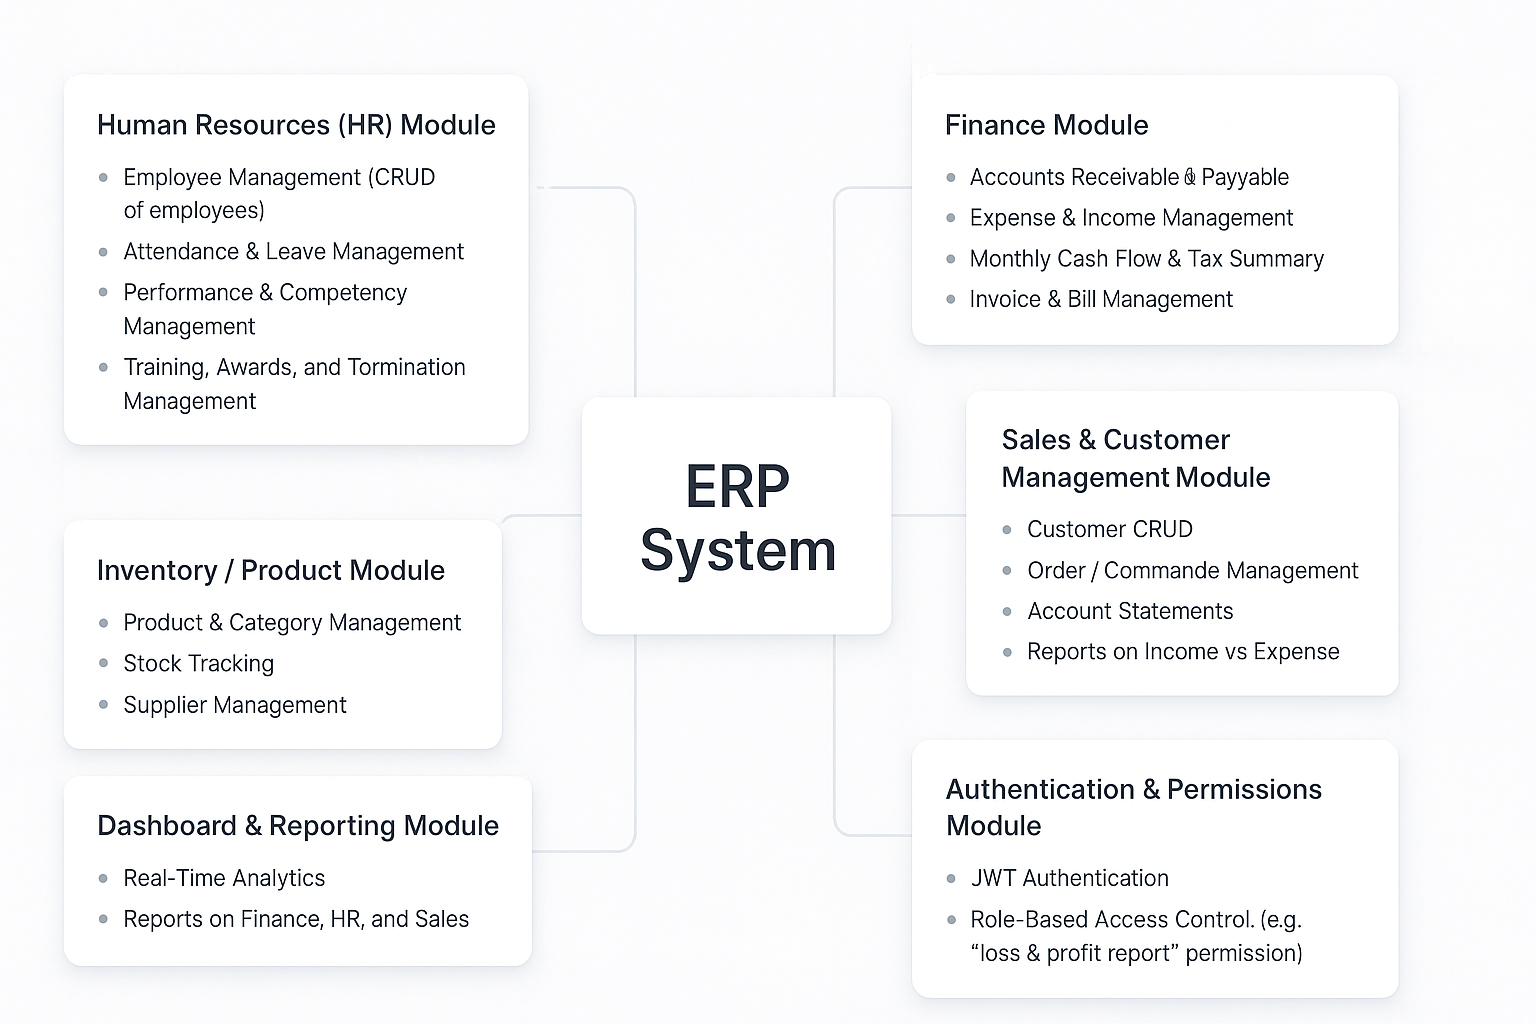
\includegraphics[width=0.7\textwidth]{chapters/chapter 1/figures/ERP_SYSTEM.png}
    \caption{High-Level Overview of the ERP System Modules}
    \label{fig:erp_modules}
\end{figure}

\section{Development Environment}
\subsection{Software Environment}
The development process was supported by a modern and efficient software toolset:
\begin{itemize}
    \item \textbf{Visual Studio Code:} Primary code editor for development.
    	\begin{figure}[H]
        \centering
        
\includegraphics[width=0.2\textwidth]{chapters/chapter 1/figures/vscode.png}
        \caption{Visual Studio Code}
        \label{fig:vscode}
    	\end{figure}
    \item \textbf{Postman:} Essential for API testing, debugging, and creating documentation for consumers.
    	\begin{figure}[H]
        \centering
        
\includegraphics[width=0.2\textwidth]{chapters/chapter 1/figures/postman.png}
        \caption{Postman API Platform}
        \label{fig:postman}
    	\end{figure}
    \item \textbf{Git \& GitLab:} Used for version control, code collaboration, and project synchronization, leveraging GitLab's integrated CI/CD and issue tracking features.
	\begin{figure}[H]
	\centering
	\begin{minipage}{0.35\textwidth}
		\centering
		
\includegraphics[width=0.6\linewidth]{chapters/chapter 1/figures/git.png}
		\subcaption{Git}
	\end{minipage}%
	\begin{minipage}{0.35\textwidth}
		\centering
		
\includegraphics[width=0.6\linewidth]{chapters/chapter 1/figures/gitLab.png}
		\subcaption{GitLab}
	\end{minipage}
	\caption{Version Control and Collaboration Tools}
	\label{fig:git_gitlab}
	\end{figure}
    \item \textbf{ClickUp:} Central hub for task management, sprint backlogs, and Agile workflow tracking.
    	\begin{figure}[H]
        \centering
        
\includegraphics[width=0.2\textwidth]{chapters/chapter 1/figures/clickUp.png}
        \caption{ClickUp Project Management}
        \label{fig:clickup}
    	\end{figure}
    \item \textbf{Overleaf / LaTeX:} Used for professional report writing, formatting, and collaborative documentation.
    	\begin{figure}[H]
        \centering
        
\includegraphics[width=0.2\textwidth]{chapters/chapter 1/figures/overleaf.jpg}
        \caption{Overleaf / LaTeX Environment}
        \label{fig:overleaf}
    	\end{figure}
   \item \textbf{PlantUML:} Used for creating UML diagrams such as use cases, class diagrams, sequence diagrams, and sequence diagrams.
    \begin{figure}[H]
        \centering
        
\includegraphics[width=0.2\textwidth]{chapters/chapter 1/figures/plantUml.png}
        \caption{PlantUML for UML Diagrams}
        \label{fig:plantuml}
    \end{figure}
\item \textbf{Draw.io:} Also employed for designing UML diagrams and system architecture visually.
    \begin{figure}[H]
        \centering
        
\includegraphics[width=0.2\textwidth]{chapters/chapter 1/figures/drawio.png}
        \caption{Draw.io for UML and Architecture Diagrams}
        \label{fig:drawio}
    \end{figure}
\item \textbf{Discord:} Platform for daily stand-ups, sprint reviews, and remote team communication.
    \begin{figure}[H]
        \centering
        
\includegraphics[width=0.2\textwidth]{chapters/chapter 1/figures/Discord-Logo.png}
        \caption{Discord Communication Platform}
        \label{fig:discord}
    \end{figure}
\end{itemize}

\subsection{Technological Choices}
The technology stack was selected to ensure performance, security, and long-term maintainability:
\begin{itemize}
    \item \textbf{Laravel:} A powerful PHP framework chosen for its elegant syntax, robust ecosystem, and built-in features that accelerate development (e.g., Eloquent ORM, Artisan).
    \item \textbf{JWT (JSON Web Tokens):} Selected for implementing stateless authentication, providing a scalable and secure way to manage user sessions across multiple devices.
    \item \textbf{MySQL:} A reliable, widely-used relational database management system ideal for handling the complex and structured data of an ERP.
    \item \textbf{REST API:} An architectural style chosen for its simplicity, statelessness, and compatibility with any front-end client (web, mobile, desktop).
    \item \textbf{LaTeX / Overleaf:} For professional, structured, and version-controlled report documentation.
    \item \textbf{PlantUML:} To programmatically generate UML diagrams ensuring maintainable and reproducible design documentation.
\end{itemize}
\begin{figure}[H]
    \centering
    % First row
    \begin{minipage}{0.45\textwidth}
        \centering
        
\includegraphics[width=\linewidth]{chapters/chapter 1/figures/laravel.png}
        \caption{Laravel}
        \label{fig:laravel}
    \end{minipage}%
    \hfill
    \begin{minipage}{0.45\textwidth}
        \centering
        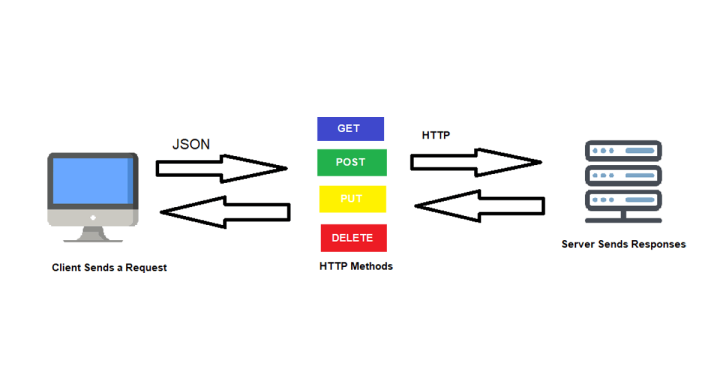
\includegraphics[width=\linewidth]{chapters/chapter 1/figures/rest-api.png}
        \caption{REST API}
        \label{fig:restapi}
    \end{minipage}

    \vspace{0.5cm} % vertical space between rows

    % Second row
    \begin{minipage}{0.45\textwidth}
        \centering
        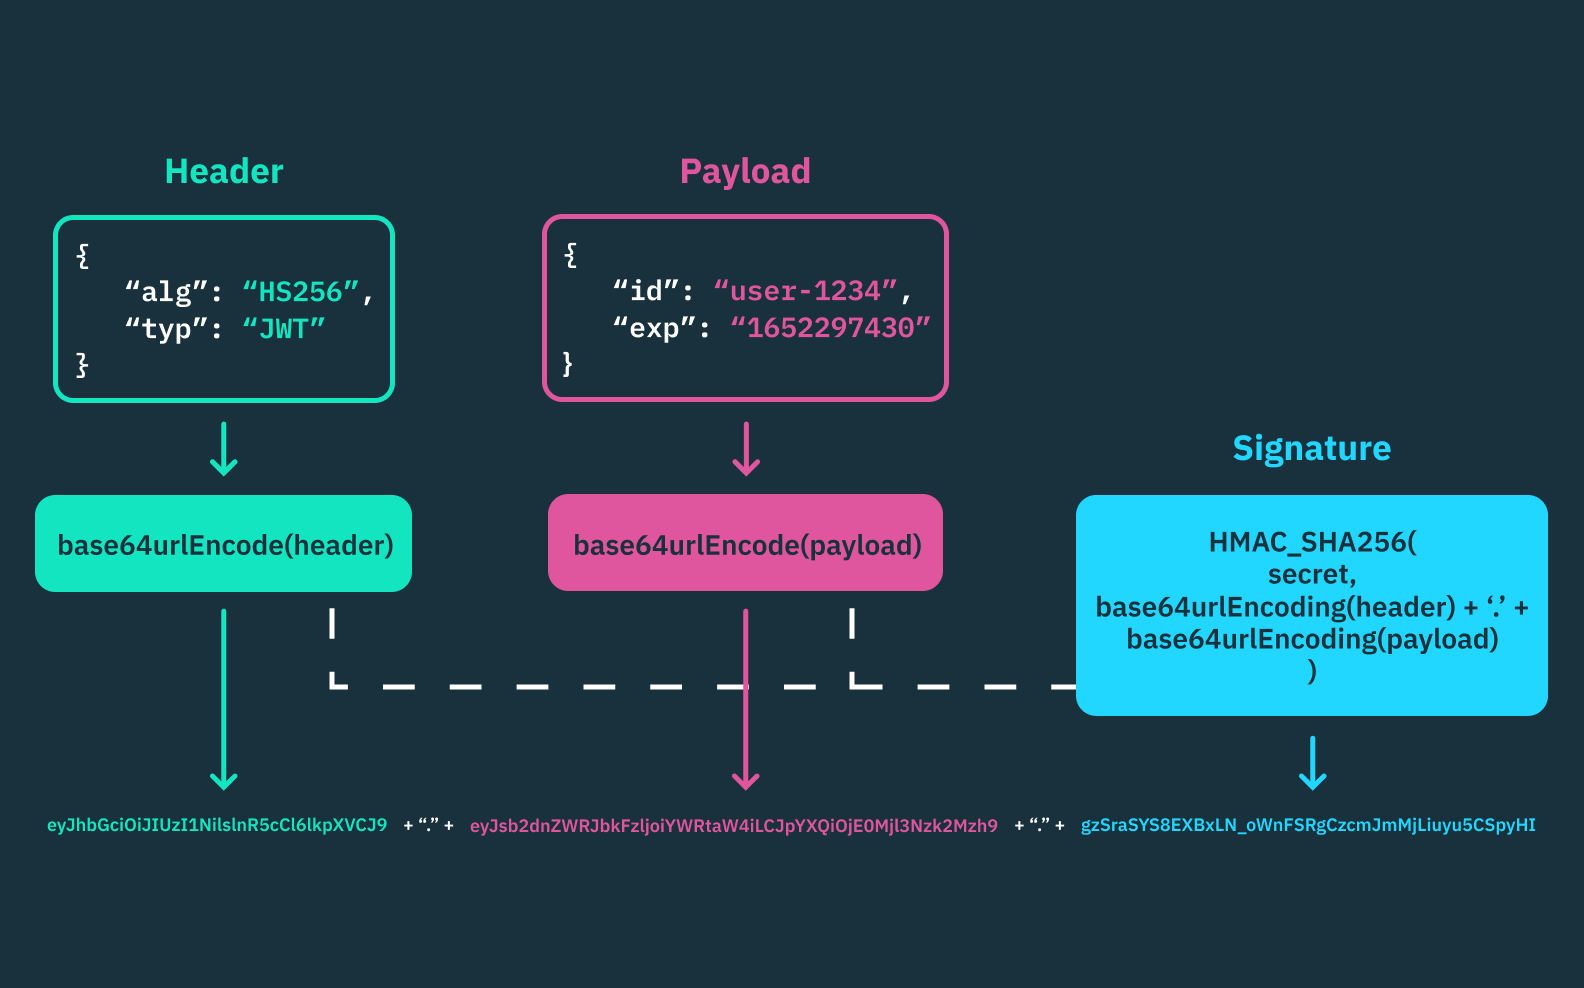
\includegraphics[width=\linewidth]{chapters/chapter 1/figures/jwt-struct.png}
        \caption{JWT}
        \label{fig:jwt}
    \end{minipage}%
    \hfill
    \begin{minipage}{0.45\textwidth}
        \centering
        
\includegraphics[width=\linewidth]{chapters/chapter 1/figures/mysql.png}
        \caption{MySQL}
        \label{fig:mysql}
    \end{minipage}
\end{figure}

\subsection{Choice of Methodology}
The project was executed using the \textbf{Agile methodology} with the \textbf{Scrum framework}. This iterative approach was crucial for managing evolving requirements, ensuring continuous delivery of value, and maintaining a high level of responsiveness to feedback.

\subsection{Presentation of the Scrum Methodology}
Scrum is an iterative Agile framework built on three pillars: \textbf{Transparency}, \textbf{Inspection}, and \textbf{Adaptation}.
\begin{itemize}
    \item \textbf{Roles:}
    \begin{itemize}
        \item \textbf{Product Owner:} Defined the project vision, managed the product backlog, and prioritized features based on business value.
        \item \textbf{Scrum Master:} Facilitated Scrum ceremonies, removed impediments, and ensured the team adhered to Agile principles.
        \item \textbf{Development Team:} Cross-functional team (myself as backend developer) responsible for designing, building, and testing the product increments.
    \end{itemize}
    \item \textbf{Events (Ceremonies):} The rhythm of the project was guided by five key events:
    \begin{itemize}
        \item \textbf{Sprint Planning:} To define the sprint goal and select backlog items for the upcoming iteration.
        \item \textbf{Daily Scrum:} A 15-minute time-boxed event for the team to synchronize activities and plan for the next 24 hours.
        \item \textbf{Sprint Review:} To inspect the increment and adapt the product backlog based on stakeholder feedback.
        \item \textbf{Sprint Retrospective:} To inspect the team's process and create a plan for improvements in the next sprint.
    \end{itemize}
\end{itemize}
\begin{figure}[H]
    \centering
    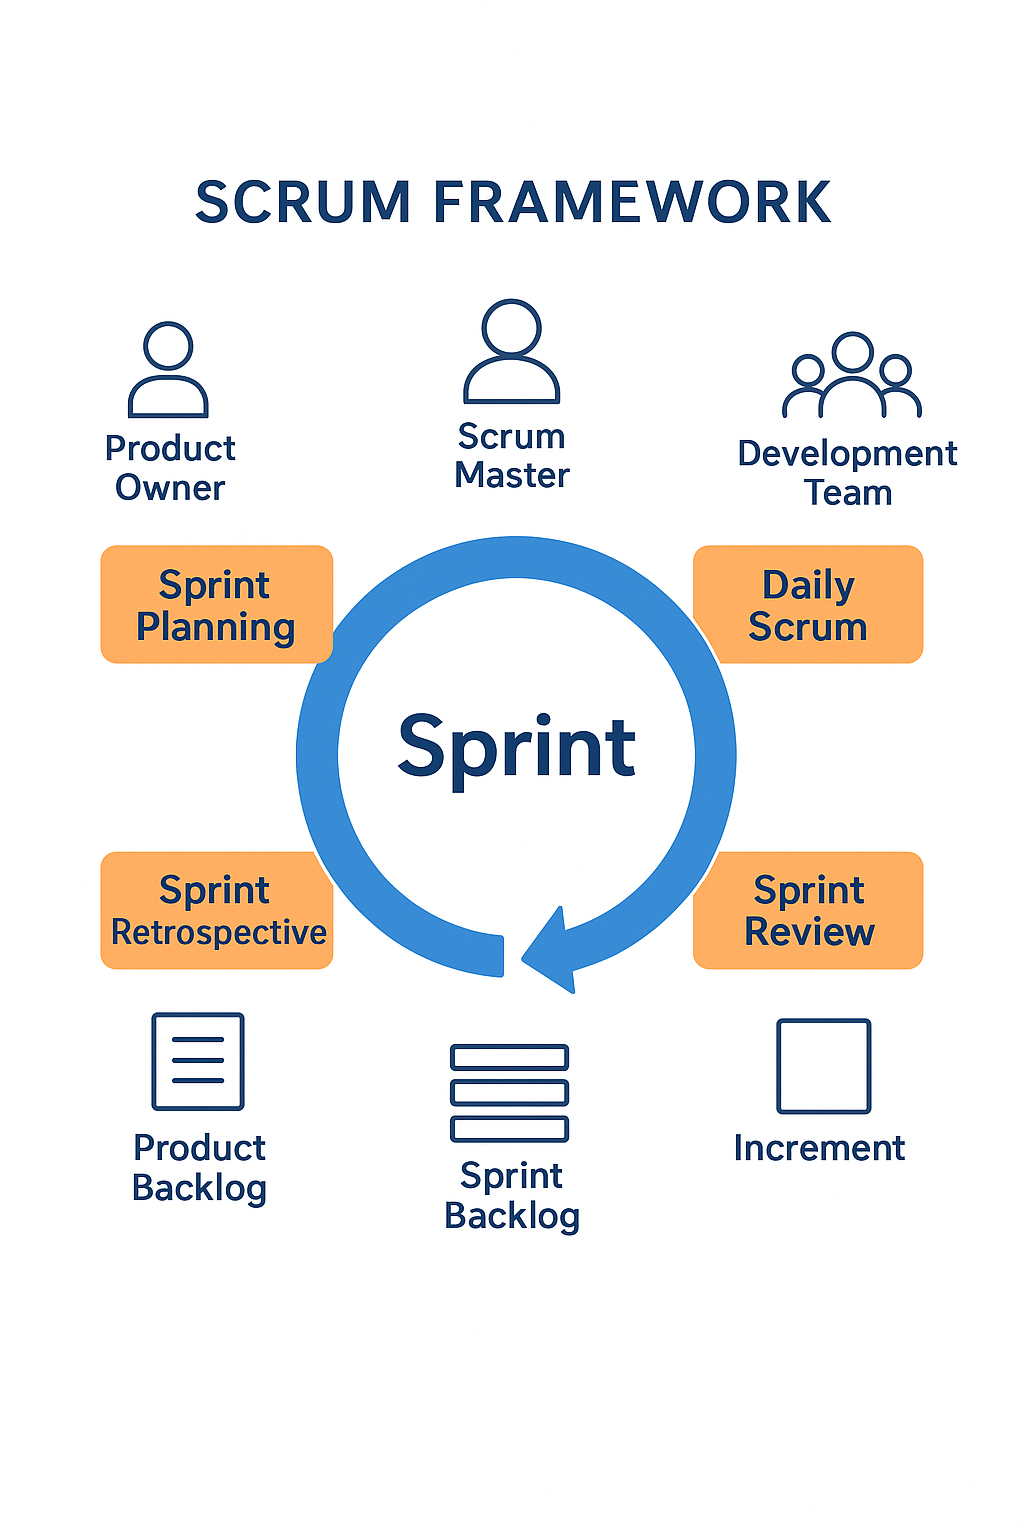
\includegraphics[width=0.9\textwidth]{chapters/chapter 1/figures/ScrumFramwork.png}
    \caption{The Scrum Framework}
    \label{fig:scrum}
\end{figure}

\section{Modeling Language}
The \textbf{Unified Modeling Language (UML)} was extensively used during the analysis and design phases to visualize, specify, and document the system's artifacts. The following diagrams were created to ensure a shared understanding of the system:
\begin{itemize}
    \item \textbf{Use Case Diagrams:} To capture functional requirements and interactions between actors and the system.
    \item \textbf{Class Diagrams:} To model the static structure of the system, showing the system's classes, attributes, methods, and relationships.
    \item \textbf{Sequence Diagrams:} To detail the dynamic interactions between objects for key processes and API calls.
    \item \textbf{Component/Architecture Diagrams:} To illustrate the high-level system components and their dependencies.
\end{itemize}
\begin{figure}[H]
    \centering
    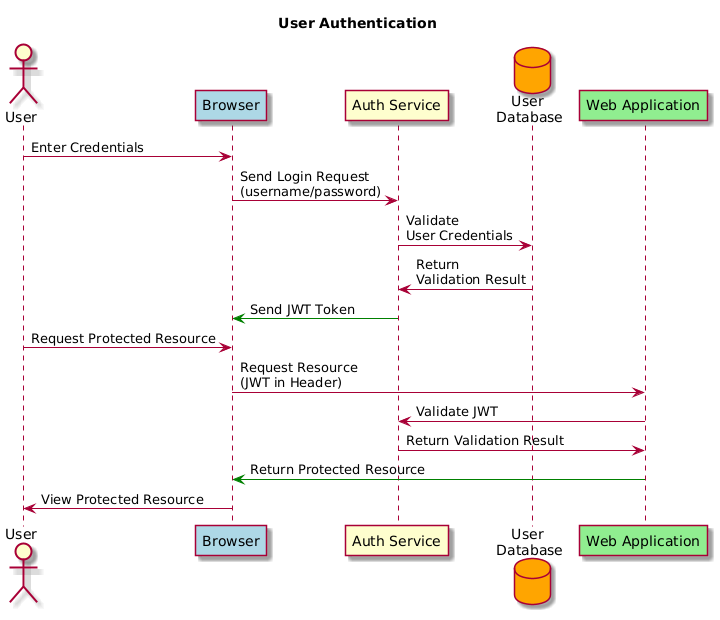
\includegraphics[width=0.7\textwidth]{chapters/chapter 1/figures/Sequence-Example2-1.png}
    \caption{Example UML Diagram (e.g., API Sequence Diagram)}
    \label{fig:uml}
\end{figure}

\section{Architecture}
The backend of the ERP system adheres to a layered \textbf{Model-View-Controller (MVC)} architecture. This promotes separation of concerns, making the codebase more organized, testable, and maintainable.
\begin{itemize}
    \item \textbf{Controller Layer:} Handles HTTP requests, invokes the necessary business logic from the Service layer, and returns appropriate HTTP responses.
    \item \textbf{Service Layer:} Contains the core business logic and rules, ensuring that controllers remain thin and logic is centralized and reusable.
    \item \textbf{Model Layer:} Utilizes Laravel's Eloquent ORM to represent business entities, manage data validation, and handle all data interactions with the database.
    \item \textbf{Database Layer:} Consists of the MySQL database, responsible for persistent and secure data storage.
\end{itemize}
This structured approach effectively separates the application's concerns, facilitating teamwork and enabling easier future enhancements.
\begin{figure}[H]
    \centering
    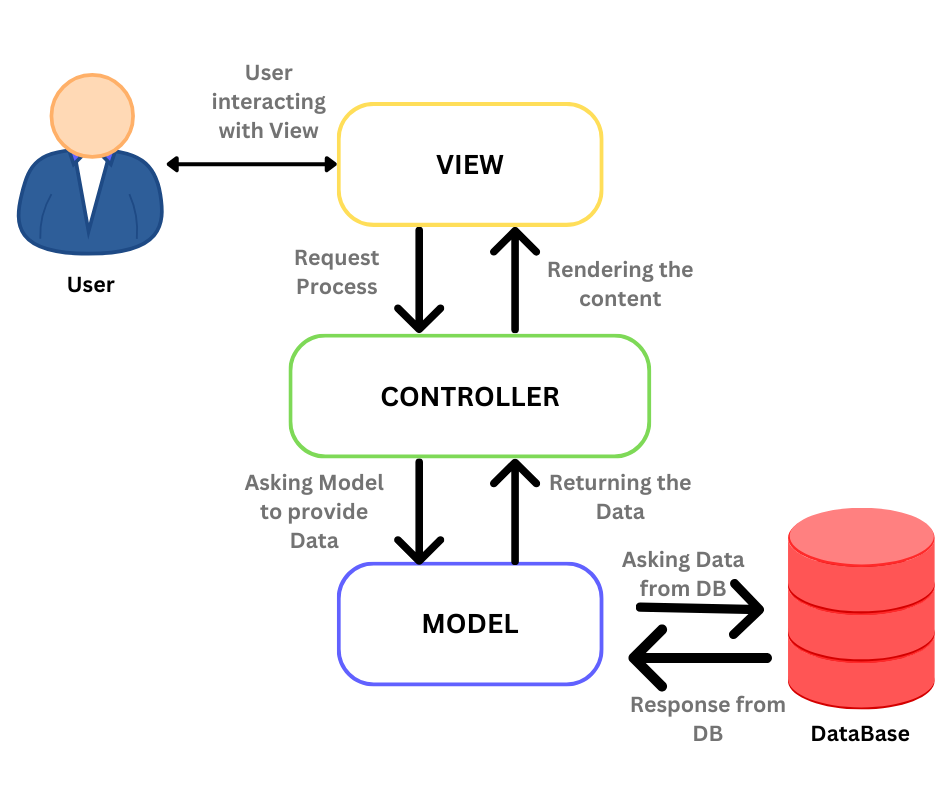
\includegraphics[width=0.8\textwidth]{chapters/chapter 1/figures/mvcArch.png}
    \caption{MVC Architecture of the Laravel Backend}
    \label{fig:mvc}
\end{figure} % Standardized naming
% Chapter 2: 
\chapter{Needs Analysis and Specification}
\minitoc % Generates a mini table of contents for this chapter

\section*{Introduction}
The success of any software project depends largely on a precise understanding of user needs and the ability to translate them into concrete specifications. 
This chapter aims to define the requirements of the ERP system developed during the internship at Anter Lab. 
It begins by identifying the key actors who will interact with the system, followed by the description of functional and non-functional requirements. 
A global use case diagram is then introduced to illustrate these interactions. 
The chapter also presents a forward-looking view of the architecture, highlighting the potential shift from a monolithic MVC structure to a microservices-based design. 
Finally, the chapter concludes with the adoption of Scrum methodology for project management, detailing the backlog and sprint planning.

\section{User needs / Capturing needs}
This chapter outlines the needs analysis and specification for the ERP system developed for Anter Lab, focusing on identifying key stakeholders, defining functional and non-functional requirements, and presenting the system's use case diagram. The analysis is grounded in the high-level module overview of the ERP system, aiming to integrate essential business processes such as human resources, accounting, customer relationship management (CRM), and point-of-sale (POS) operations for small and medium-sized enterprises (SMEs).

\subsection{Identifying key players}
The ERP system involves multiple actors who interact with its various modules. Based on the system architecture and discussions with stakeholders during the internship, the primary actors are:

\begin{itemize}
    \item \textbf{Super Admin}: Has full control over the system, manages global settings, oversees all users and modules.
    \item \textbf{Admin}: Responsible for system-wide management, including authentication, user management, settings, and configuration.
    \item \textbf{Employee/User}: Engages with human resource management (HRM), project tracking, task management, and support features.
    \item \textbf{Manager}: Oversees CRM, accounting, POS, product management, and project oversight.
    \item \textbf{Client}: Interacts with project consultation, contract management, timesheets, and support services.
    \item \textbf{External Services}: APIs for third-party integrations (Zoom, Slack, Telegram, Payment gateways).
\end{itemize}

These actors were identified through a detailed analysis of the ERP module hierarchy and stakeholder feedback.

\subsection{Functional requirements}
The functional requirements specify the core functionalities the ERP system must provide, categorized by module based on the system design:

\begin{itemize}
    \item \textbf{Authentication}: Enable user login, registration, credential verification, and password reset with JWT security.
    \item \textbf{HRM Management}: Manage employee appraisals, recruitment, onboarding, attendance, leave, payroll, and collaboration events.
    \item \textbf{Accounting Management}: Handle purchasing, expenses, sales, budgeting, planning, and core accounting tasks.
    \item \textbf{CRM Management}: Support lead lifecycle management, deal pipelines, contract handling, feedback collection, and CRM configuration.
    \item \textbf{Project Management}: Facilitate project tracking, task assignment, and timesheet management.
    \item \textbf{User Management}: Provide user account creation, role assignment, permissions, and notifications.
    \item \textbf{Product Management}: Track product stock, manage pricing, and control warehouse and inventory.
    \item \textbf{POS Management}: Manage quotations, POS transactions, purchases, and transfer operations.
    \item \textbf{Support Management}: Integrate communication tools like Zoom, Telegram, Chat, and Slack for support services.
    \item \textbf{Settings Management}: Allow configuration of login settings and general system parameters.
    \item \textbf{Client Features}: Enable clients to consult projects, contracts, timesheets, calendars, tasks, bugs, and support requests.
    \item \textbf{Notification System}: Send real-time alerts for HR, accounting, CRM, or system activities.
    \item \textbf{Audit Logging}: Track all system actions for compliance and debugging.
    \item \textbf{Reporting \& Analytics}: Generate reports for HRM, Accounting, CRM, and POS modules.
    \item \textbf{Integration Layer}: Allow external APIs (e.g., payment gateways) to communicate with the ERP.
\end{itemize}

These requirements ensure comprehensive coverage of SME business processes.

\subsection{Non-functional requirements}
The non-functional requirements define the system's quality attributes to ensure reliability and usability:

\begin{itemize}
    \item \textbf{Security}: Implement JWT authentication to secure all API endpoints and protect sensitive data.
    \item \textbf{Performance}: Ensure API responses within 2 seconds under typical load, with optimized MySQL queries.
    \item \textbf{Scalability}: Support up to 100 concurrent users, with a modular design for future growth.
    \item \textbf{Usability}: Provide intuitive APIs with Postman documentation, supporting web and mobile interfaces.
    \item \textbf{Reliability}: Achieve 99\% uptime with robust error handling and logging in Laravel.
    \item \textbf{Maintainability}: Adhere to MVC architecture for easy updates, using Git for version control.
    \item \textbf{Auditability}: Keep secure logs of critical operations for compliance.
    \item \textbf{Data Backup \& Recovery}: Ensure automatic daily backups and quick recovery procedures.
    \item \textbf{Continuous Integration/Delivery (CI/CD)}: Use GitLab pipelines for automated testing and deployment.
\end{itemize}

These attributes guarantee a robust and adaptable system.

\subsection{Overall Use Case Diagram}
The overall use case diagram illustrates the interactions between actors and the ERP system's functionalities. This diagram is derived from the module hierarchy and functional requirements outlined above.

\begin{figure}[H]
    \centering
    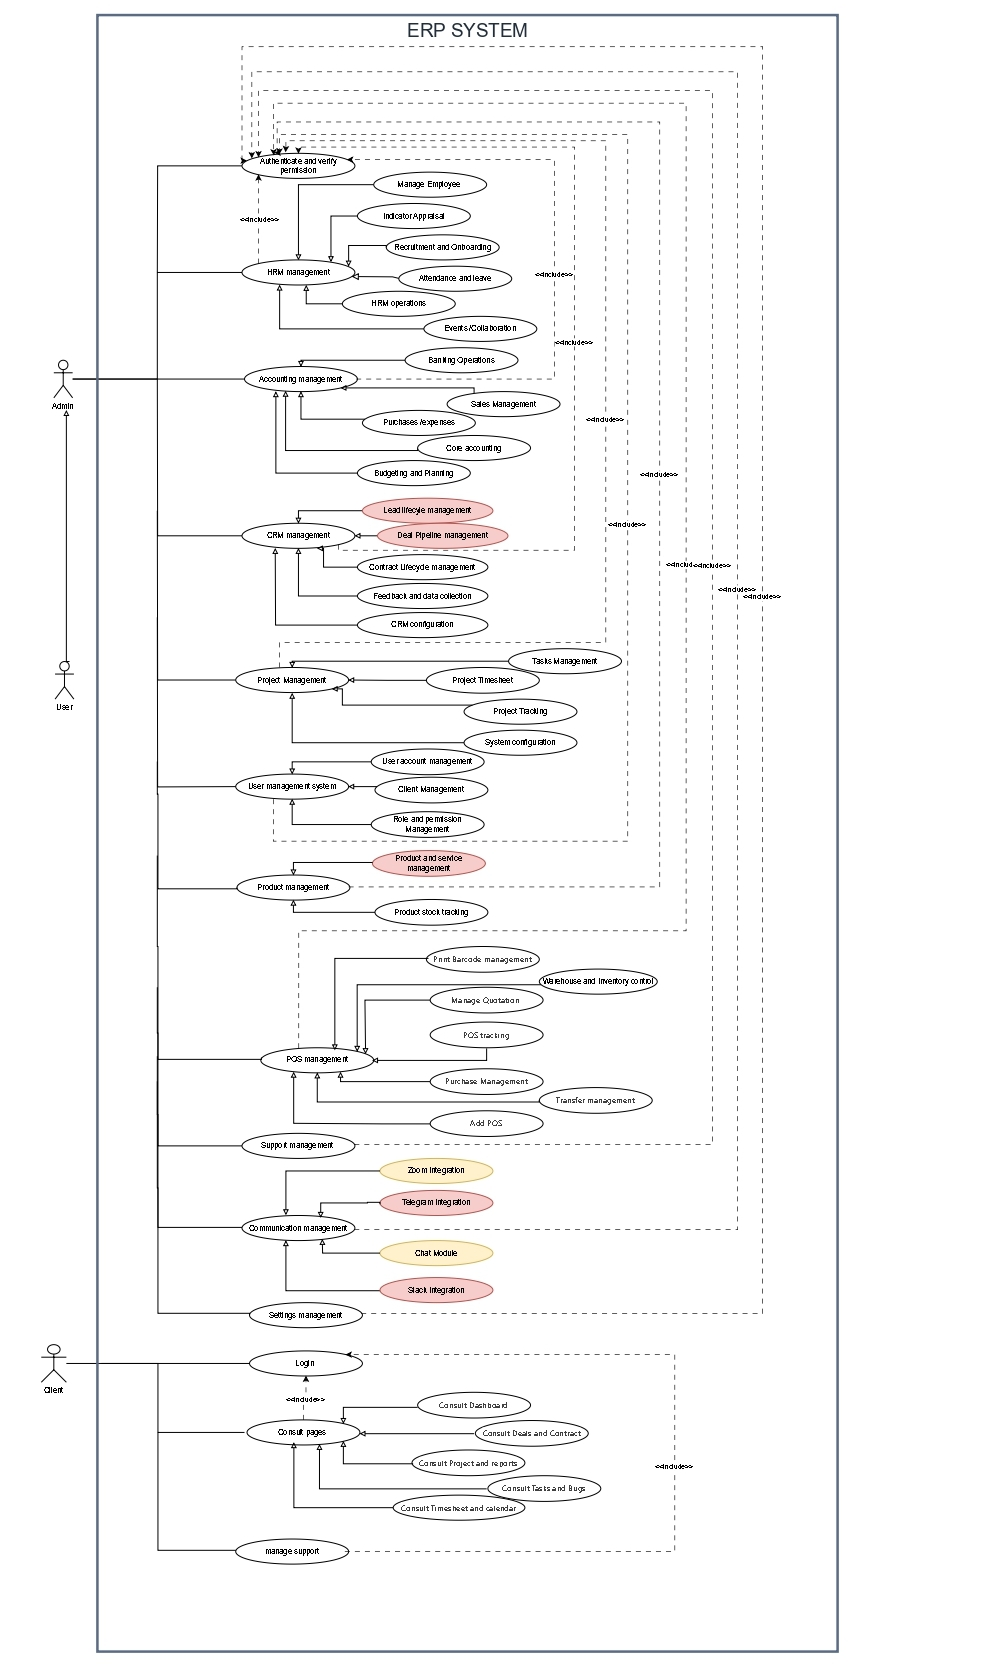
\includegraphics[width=0.9\textwidth]{chapters/chapter 2/figures/diagramGeneralUseCase (1) (1).drawio (1)_page-0001 (1).jpg}
    \caption{Overall Use Case Diagram of the ERP System}
    \label{fig:overall_use_case}
\end{figure}

\subsection{Micro-services Architecture}
While the current implementation follows a monolithic MVC architecture using Laravel, a future transition to a microservices architecture is considered for enhanced scalability. Each module (e.g., HRM, CRM, POS) could operate as an independent service, communicating via REST APIs.

\begin{figure}[H]
    \centering
    \begin{tikzpicture}[
        node distance=1.5cm and 2cm,
        service/.style={
            draw, 
            rectangle, 
            rounded corners=4pt,
            minimum width=3cm, 
            minimum height=1.5cm,
            align=center,
            text width=2.8cm,
            font=\small,
            fill=green!10
        },
        gateway/.style={
            service,
            fill=blue!10,
            minimum width=4cm
        },
        db/.style={
            service,
            fill=gray!10,
            minimum height=2cm
        },
        arrow/.style={
            ->,
            thick,
            shorten >=2pt,
            shorten <=2pt
        }
    ]
        % API Gateway (Central Hub)
        \node[gateway] (api_gateway) {API Gateway};
        
        % Microservices
        \node[service, below=of api_gateway, xshift=-4cm] (auth_service) {Authentication Service};
        \node[service, below=of api_gateway] (hrm_service) {HRM Service};
        \node[service, below=of api_gateway, xshift=4cm] (crm_service) {CRM Service};
        \node[service, below=of hrm_service, xshift=-4cm] (pos_service) {POS Service};
        \node[service, below=of hrm_service] (accounting_service) {Accounting Service};
        \node[service, below=of hrm_service, xshift=4cm] (user_service) {User Management Service};
        \node[service, below=of accounting_service, xshift=-2cm] (product_service) {Product Management Service};
        \node[service, below=of accounting_service, xshift=2cm] (support_service) {Support Service};
        
        % Database Layer
        \node[db, below=of support_service, xshift=0cm] (database) {Central Database (MySQL)};
        
        % Arrows from Gateway to Services
        \draw[arrow] (api_gateway) -- (auth_service);
        \draw[arrow] (api_gateway) -- (hrm_service);
        \draw[arrow] (api_gateway) -- (crm_service);
        \draw[arrow] (api_gateway) -| (pos_service);
        \draw[arrow] (api_gateway) -| (accounting_service);
        \draw[arrow] (api_gateway) -| (user_service);
        \draw[arrow] (api_gateway) -| (product_service);
        \draw[arrow] (api_gateway) -| (support_service);
        
        % Arrows from Services to Database
        \draw[arrow] (auth_service) -- (database);
        \draw[arrow] (hrm_service) -- (database);
        \draw[arrow] (crm_service) -- (database);
        \draw[arrow] (pos_service) -- (database);
        \draw[arrow] (accounting_service) -- (database);
        \draw[arrow] (user_service) -- (database);
        \draw[arrow] (product_service) -- (database);
        \draw[arrow] (support_service) -- (database);
    \end{tikzpicture}
    \caption{Microservices Architecture Overview}
    \label{fig:microservices}
\end{figure}

\section{Project management with Scrum}
The development process adopts the Scrum methodology to manage iterative progress, ensuring flexibility and regular feedback.

\subsection{Product backlog}
The product backlog contains prioritized user stories to guide sprint planning:

\begin{longtable}{|p{3cm}|p{5cm}|p{3cm}|p{2cm}|}
\hline
\textbf{User Story} & \textbf{Description} & \textbf{Priority} & \textbf{Estimate} \\
\hline
\endfirsthead
\hline
\textbf{User Story} & \textbf{Description} & \textbf{Priority} & \textbf{Estimate} \\
\hline
\endhead
As a Super Admin, I want to configure system-wide parameters. & Manage ERP modules, integrations, and roles globally. & High & 8 \\
\hline
As an Admin, I want to authenticate users with JWT. & Implement secure login, registration, and verification. & High & 5 \\
\hline
As a Manager, I want to manage HRM functions. & CRUD for appraisals, recruitment, attendance. & High & 8 \\
\hline
As a Manager, I want to handle accounting tasks. & Manage purchases, sales, budgeting. & Medium & 7 \\
\hline
As a Manager, I want to manage CRM leads. & Lead lifecycle, deal pipelines, contracts. & Medium & 6 \\
\hline
As an Employee, I want to track projects. & Task assignment, timesheets, tracking. & High & 5 \\
\hline
As an Admin, I want to manage user accounts. & Role assignment, permissions, notifications. & High & 4 \\
\hline
As a Manager, I want to manage products. & Stock, pricing, inventory control. & Medium & 6 \\
\hline
As a Manager, I want to handle POS operations. & Quotations, purchases, transfers. & Medium & 5 \\
\hline
As an Employee, I want support integrations. & Zoom, Telegram, Chat, Slack. & Low & 3 \\
\hline
As a Client, I want to consult project details. & View projects, contracts, timesheets. & Medium & 4 \\
\hline
As an Admin, I want to see system audit logs. & Track sensitive actions for compliance. & High & 6 \\
\hline
As a Manager, I want reporting dashboards. & Generate HR, CRM, Accounting KPIs. & Medium & 7 \\
\hline
As a Developer, I want CI/CD pipelines. & Automate testing and deployment with GitLab. & High & 5 \\
\hline
\caption{Product Backlog}
\label{tab:product_backlog}
\end{longtable}

\subsection{Sprint Planning}
The internship project was organized using the \textbf{Scrum framework}, with weekly sprints due to the one-month duration. Each sprint was carefully planned with specific objectives to ensure steady progress and incremental delivery.

\begin{longtable}{|p{1.5cm}|p{4cm}|p{2.5cm}|p{5.5cm}|}
\hline
\textbf{Sprint} & \textbf{Objective} & \textbf{Duration} & \textbf{Main Tasks (Planned)} \\
\hline
\endfirsthead
\hline
\textbf{Sprint} & \textbf{Objective} & \textbf{Duration} & \textbf{Main Tasks (Planned)} \\
\hline
\endhead
\textbf{Sprint 0} & Project setup and team onboarding & Week 1 & 
\begin{itemize}
    \item Clone and run project locally from GitLab
    \item Configure database and run migrations
    \item Join ClickUp workspace and Discord server
    \item Setup backend foundation (API scaffolding)
    \item Implement initial APIs: Register, Login, getUserInfo
    \item Migrate Dashboard Controller to API version
\end{itemize} \\
\hline
\textbf{Sprint 1} & Core administrative APIs & Week 2 & 
\begin{itemize}
    \item CRUD operations for Employees (with Import/Export)
    \item CRUD operations for Branches
    \item CRUD operations for Departments
    \item CRUD operations for Designations
\end{itemize} \\
\hline
\textbf{Sprint 2} & Configuration \& Option Management APIs & Week 3 & 
\begin{itemize}
    \item Leave Type, Document Type, Payslip Type APIs
    \item Allowance Option, Loan Option, Deduction Option APIs
    \item Goal Type, Training Type, Award Type APIs
    \item Termination Type, Job Category, Job Stage APIs
    \item Performance Type, Competencies APIs
\end{itemize} \\
\hline
\textbf{Sprint 3} & Reporting \& Data Export APIs & Week 4 & 
\begin{itemize}
    \item Financial Summary Reports: Income, Expense, Cash Flow, Tax
    \item Transaction Reports: Invoices, Sales, Purchases, Receivables/Payables
    \item Inventory, Ledger, and Account Statement reports
    \item Data Export APIs for all reports
\end{itemize} \\
\hline
\caption{Sprint Planning Overview}
\label{tab:sprint_planning}
\end{longtable}

\section*{Conclusion}
In summary, this chapter established a solid foundation for the ERP system by identifying stakeholders, capturing functional and non-functional requirements, and illustrating the interactions through use case diagrams. 
The analysis highlighted not only the core modules (HRM, Accounting, CRM, POS, etc.) but also additional cross-cutting concerns such as authentication, reporting, and integration with external services. 
Furthermore, non-functional requirements such as security, scalability, and maintainability were emphasized to ensure the system’s robustness. 
The sprint planning section provided a roadmap for iterative development using the Scrum framework, ensuring that progress could be tracked weekly and objectives refined based on feedback. 
This detailed specification phase paves the way for the implementation stage, which will be covered in Chapter 3, focusing on the execution of each sprint.

%Chapter 2 :
\chapter{Implementation and Realization}
\minitoc % Generates a mini table of contents for this chapter

\section*{Introduction}
This chapter presents the implementation of the ERP backend system carried out during the internship at Anter Lab. 
The work followed the Scrum methodology, divided into four weekly sprints due to the one-month duration of the internship. 
Each sprint focused on specific objectives: environment setup, core administrative APIs, configuration management, and reporting. 
In addition, we illustrate the design with UML diagrams (use case, class, sequence) and provide scenario tables for selected modules.

% Include each sprint file
\section{Sprint 0: Environment \& Project Setup}

\subsection{Objectives}
Sprint 0 was dedicated to laying the groundwork for the ERP backend system. 
The main goal was to establish a stable and collaborative development environment, ensuring all team members shared the same technical foundation. 
This sprint also introduced initial API scaffolding, which served as the backbone for future sprints.

\subsection{Tasks Completed}

\paragraph{1. Project Initialization and Source Control}
\begin{itemize}
    \item Cloned the ERP backend project from the private GitLab repository.
    \item Verified and configured the development branch, ensuring proper synchronization with GitLab’s version control system.
    \item Established branching strategy (\texttt{main}, \texttt{develop}, feature branches) to support parallel work.
\end{itemize}

\paragraph{2. Environment and Database Setup}
\begin{itemize}
    \item Installed necessary dependencies for Laravel and PHP (via Composer).
    \item Configured the \texttt{.env} file for database connection and environment-specific settings.
    \item Created and migrated the MySQL database schema.
    \item Seeded initial data (roles, admin user) for authentication testing.
\end{itemize}

\paragraph{3. Communication and Project Management Tools}
\begin{itemize}
    \item Joined the ClickUp workspace, where the product backlog and sprint tasks were organized.
    \item Integrated into the Discord server for team communication, enabling daily stand-ups and instant collaboration.
    \item Defined the workflow of tracking tasks (To Do, In Progress, Done).
\end{itemize}

\paragraph{4. API Foundations}
\begin{itemize}
    \item Migrated the legacy \texttt{DashboardController} into REST API endpoints to align with modern backend architecture.
    \item Developed the first set of APIs:
    \begin{itemize}
        \item \texttt{POST /register} – User registration endpoint.
        \item \texttt{POST /login} – JWT-based authentication endpoint.
        \item \texttt{GET /user-info} – Fetch authenticated user profile and roles.
    \end{itemize}
    \item Documented these endpoints and tested them in Postman.
\end{itemize}

\subsection{Outputs}
By the end of Sprint 0, the following deliverables were achieved:
\begin{itemize}
    \item A fully functional Laravel project running locally with database integration.
    \item Secure JWT authentication flow in place (Register, Login, User Info).
    \item A collaborative workflow using GitLab (source control), ClickUp (task management), and Discord (communication).
    \item A clear project roadmap established through backlog prioritization.
\end{itemize}

% --------------------------------------------------------
% USE CASE DIAGRAM
% --------------------------------------------------------
\subsection{Authentication Use Case Diagram}
\begin{figure}[H]
    \centering
    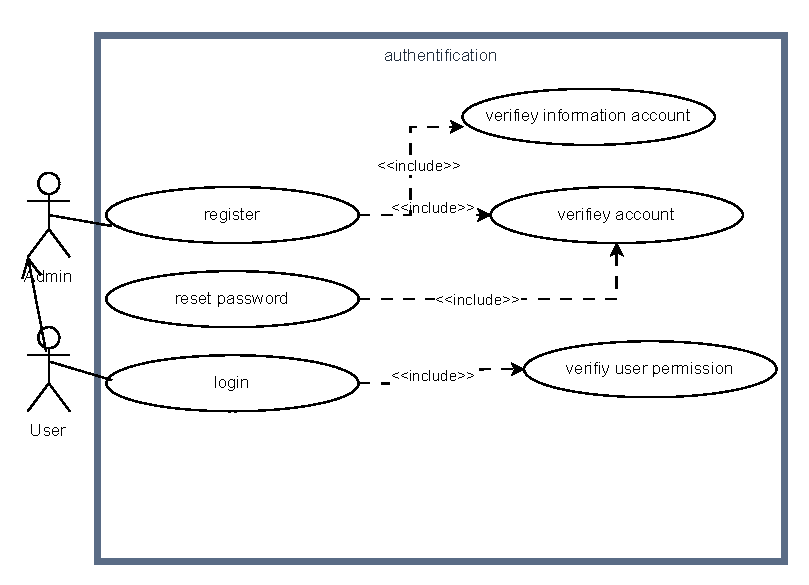
\includegraphics[width=0.85\textwidth]{chapters/chapter 3/figures/AuthUseCase.drawio_cropped.pdf}
    \caption{Specific Use Case Diagram for Authentication APIs}
    \label{fig:sprint0_usecase}
\end{figure}

% --------------------------------------------------------
% USE CASE SCENARIO TABLE
% --------------------------------------------------------
\subsection{Use Case Scenario: User Login}
\begin{longtable}{|p{3cm}|p{11cm}|}
\hline
\textbf{Use Case} & User Login with JWT \\
\hline
\textbf{Actor} & Registered User \\
\hline
\textbf{Preconditions} & 
\begin{minipage}[t]{10cm}
\begin{itemize}
    \item User already registered in the system.
    \item Database contains valid user credentials.
\end{itemize}
\end{minipage} \\
\hline
\textbf{Main Flow} &
\begin{minipage}[t]{10cm}
\begin{enumerate}
    \item User enters email and password.
    \item System verifies credentials against database.
    \item If valid, system generates JWT token.
    \item System returns token and user details to client.
\end{enumerate}
\end{minipage} \\
\hline
\textbf{Alternative Flows} &
\begin{minipage}[t]{10cm}
\begin{itemize}
    \item Invalid credentials → System returns error message.
    \item Missing data → System prompts user to re-enter credentials.
\end{itemize}
\end{minipage} \\
\hline
\textbf{Postconditions} & 
\begin{minipage}[t]{10cm}
User is authenticated, token stored for accessing protected APIs.
\end{minipage} \\
\hline
\caption{Use Case Scenario: User Login}
\label{tab:usecase_login}
\end{longtable}
% --------------------------------------------------------
% SEQUENCE DIAGRAM
% --------------------------------------------------------
\subsection{Sequence Diagram: User Login Flow}
\begin{figure}[H]
    \centering
    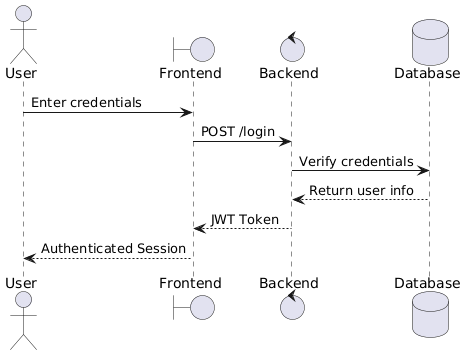
\includegraphics[width=0.9\textwidth]{chapters/chapter 3/figures/sequence_DG_Auth.png}
    \caption{Sequence Diagram for Login API}
    \label{fig:sprint0_sequence}
\end{figure}

% --------------------------------------------------------
% CLASS DIAGRAM
% --------------------------------------------------------
\subsection{Class Diagram: Authentication Module}
\begin{figure}[H]
    \centering
    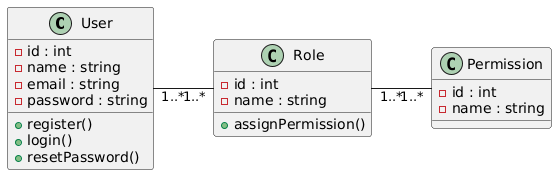
\includegraphics[width=0.85\textwidth]{chapters/chapter 3/figures/class_diagram.png}
    \caption{Class Diagram for Authentication Entities}
    \label{fig:sprint0_class}
\end{figure}

\subsection{API Testing with Postman}
To validate the core authentication APIs, Postman was used for sending HTTP requests and verifying responses. The following figures illustrate the results of the \texttt{Register}, \texttt{Login}, and \texttt{/user} (getUserInfo) endpoints.

\begin{figure}[H]
    \centering
    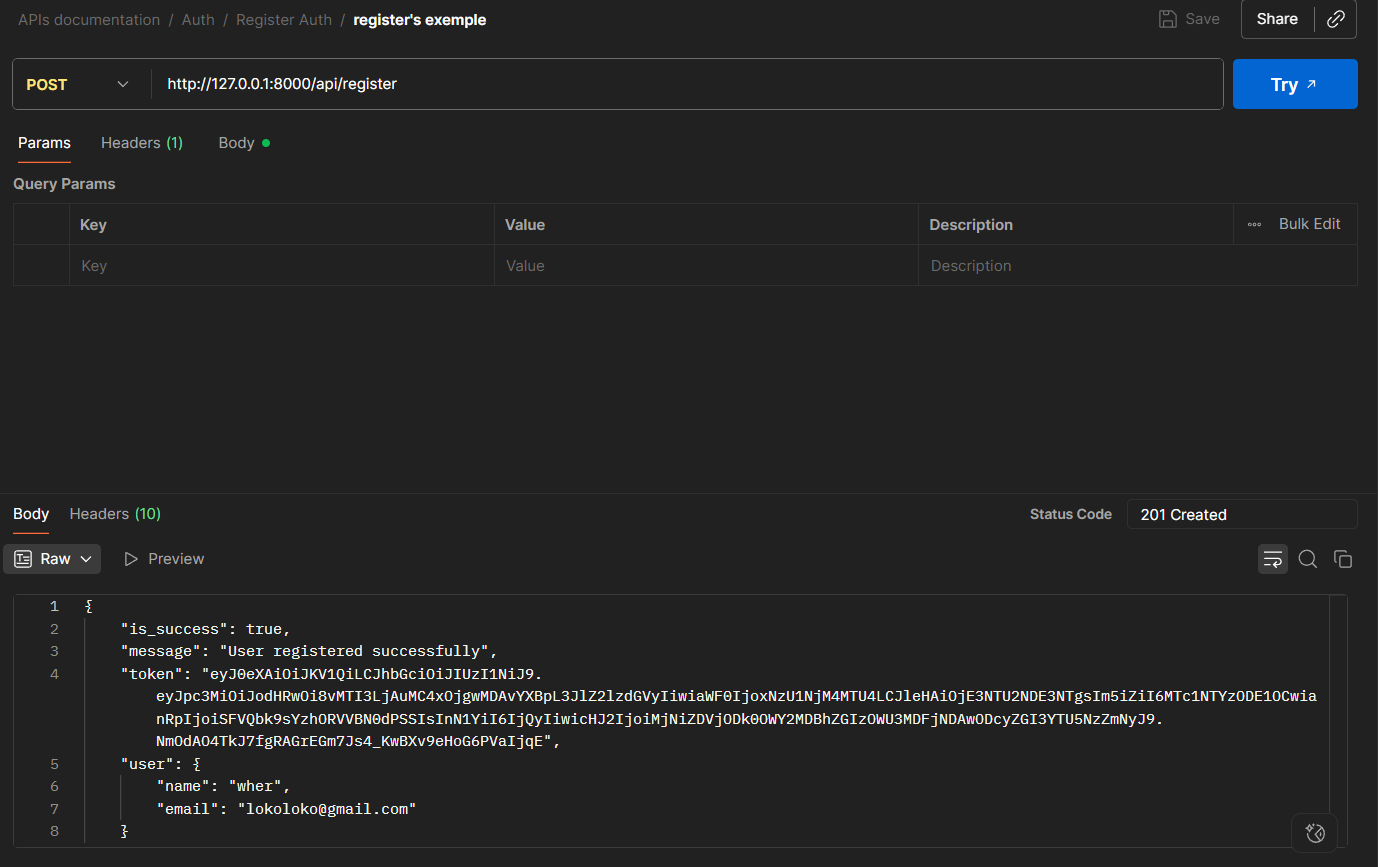
\includegraphics[width=0.8\textwidth]{chapters/chapter 3/figures/register.png}
    \caption{Postman Test -- Register API (Successful User Registration)}
    \label{fig:postman_register}
\end{figure}

\begin{figure}[H]
    \centering
    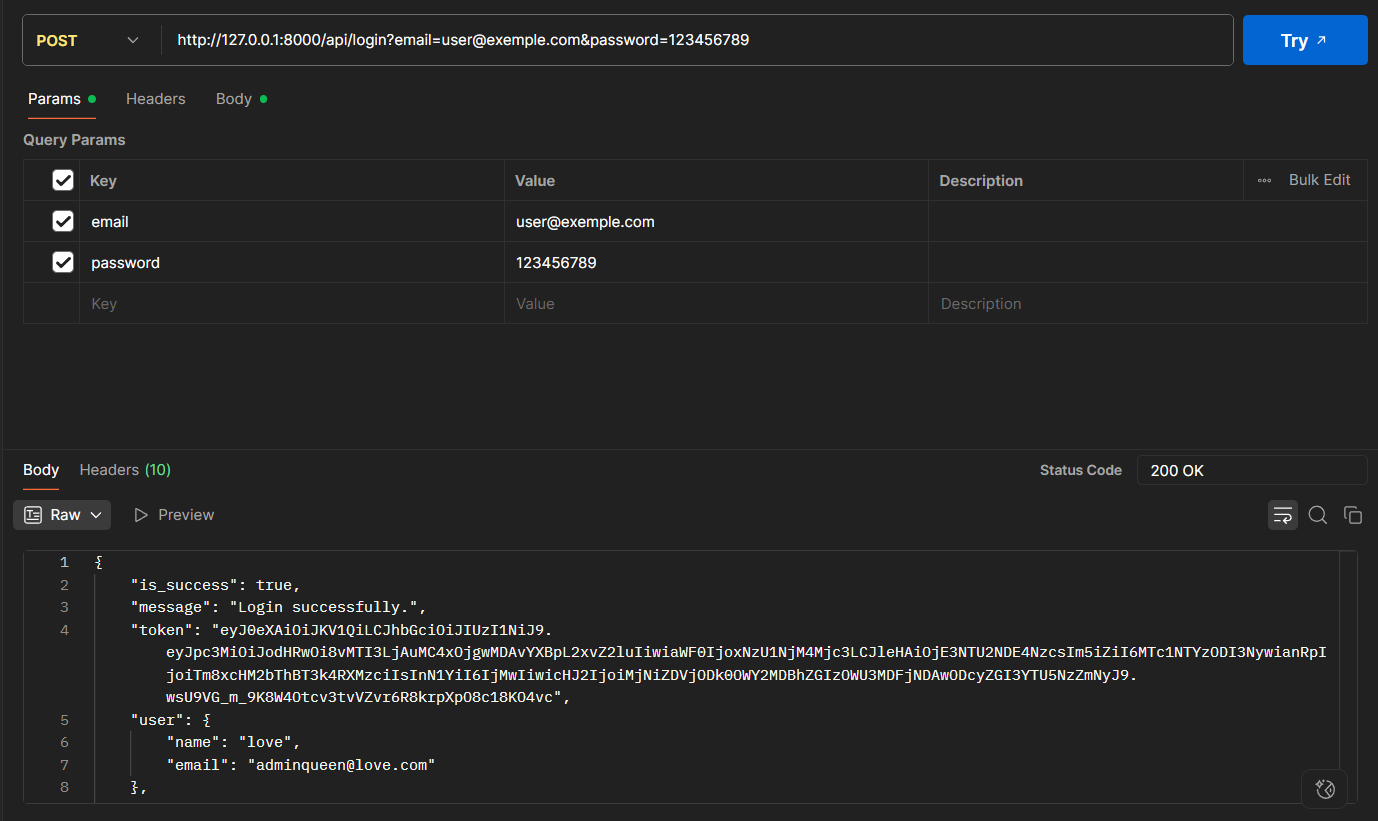
\includegraphics[width=0.8\textwidth]{chapters/chapter 3/figures/login.png}
    \caption{Postman Test -- Login API (Authentication with JWT)}
    \label{fig:postman_login}
\end{figure}

\begin{figure}[H]
    \centering
    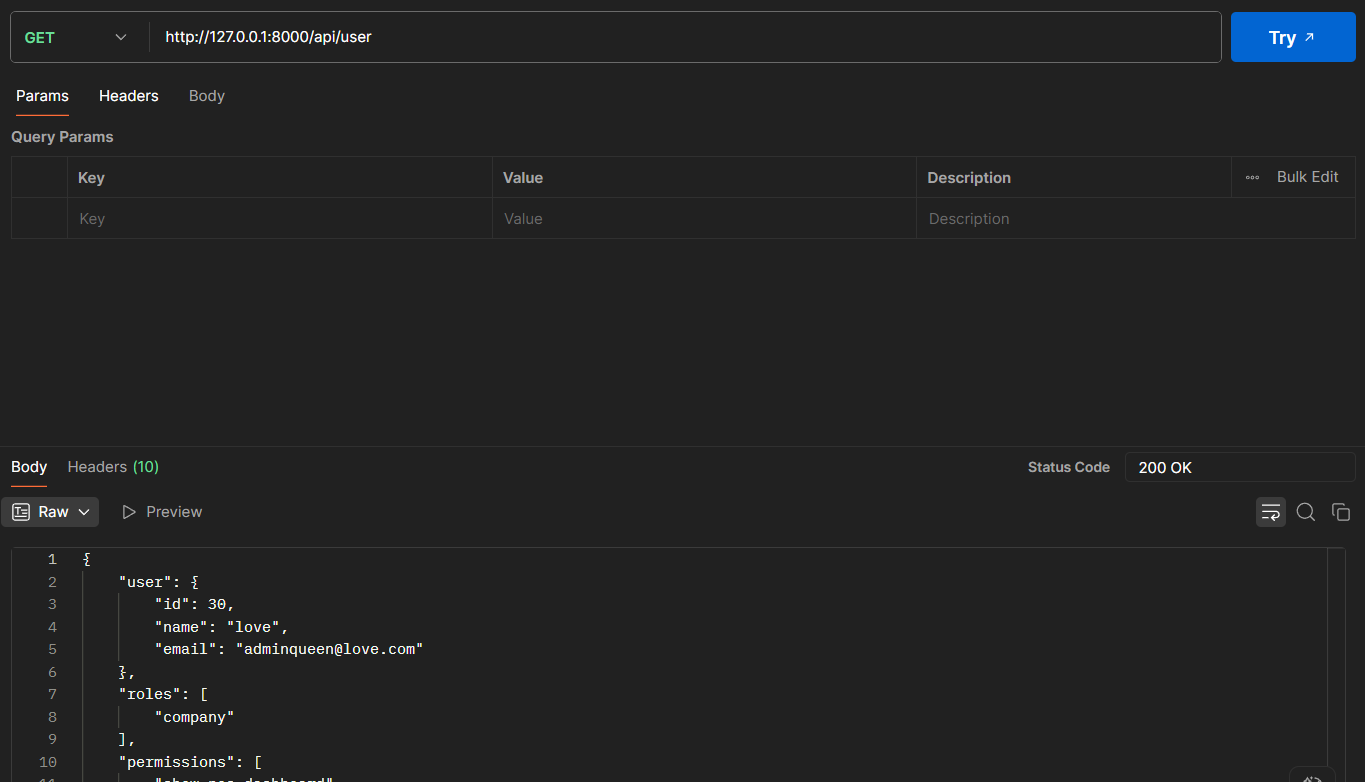
\includegraphics[width=0.8\textwidth]{chapters/chapter 3/figures/user.png}
    \caption{Postman Test -- /user API (Fetching Authenticated User Information)}
    \label{fig:postman_user}
\end{figure}

\section{Sprint 0: Dashboard API Endpoints (HRM Example)}

\subsection{Objectives}
The objective of this part of Sprint 0 was to migrate the legacy Dashboard features into REST API endpoints and make them available for the ERP backend.  
The dashboard contains several modules such as HRM, POS, CRM, Accounting, and general system monitoring. In this section, we focus on the HRM (Human Resources Management) dashboard as a representative example.

\subsection{Main Endpoints (Dashboard APIs)}
The following endpoints were implemented and tested in Sprint 0:
\begin{itemize}
    \item \texttt{GET /dashboard-index} – Main dashboard overview.
    \item \texttt{GET /crm-dashboard} – CRM module summary.
    \item \texttt{GET /hrm-dashboard} – HRM module summary.
    \item \texttt{GET /pos-dashboard} – POS (Point of Sale) overview.
    \item \texttt{GET /account-dashboard-index} – Accounting/Finance summary.
    \item \texttt{GET /order-chart} – Charts for orders and transactions.
    \item \texttt{GET /get-projects} – Projects overview.
\end{itemize}

\subsection{Use Case: HRM Dashboard}
The HRM dashboard aggregates employee management, payroll, attendance, and recruitment data for managers and admins. Figure~\ref{fig:hrm_use_case} shows the use case diagram.

\begin{figure}[H]
    \centering
    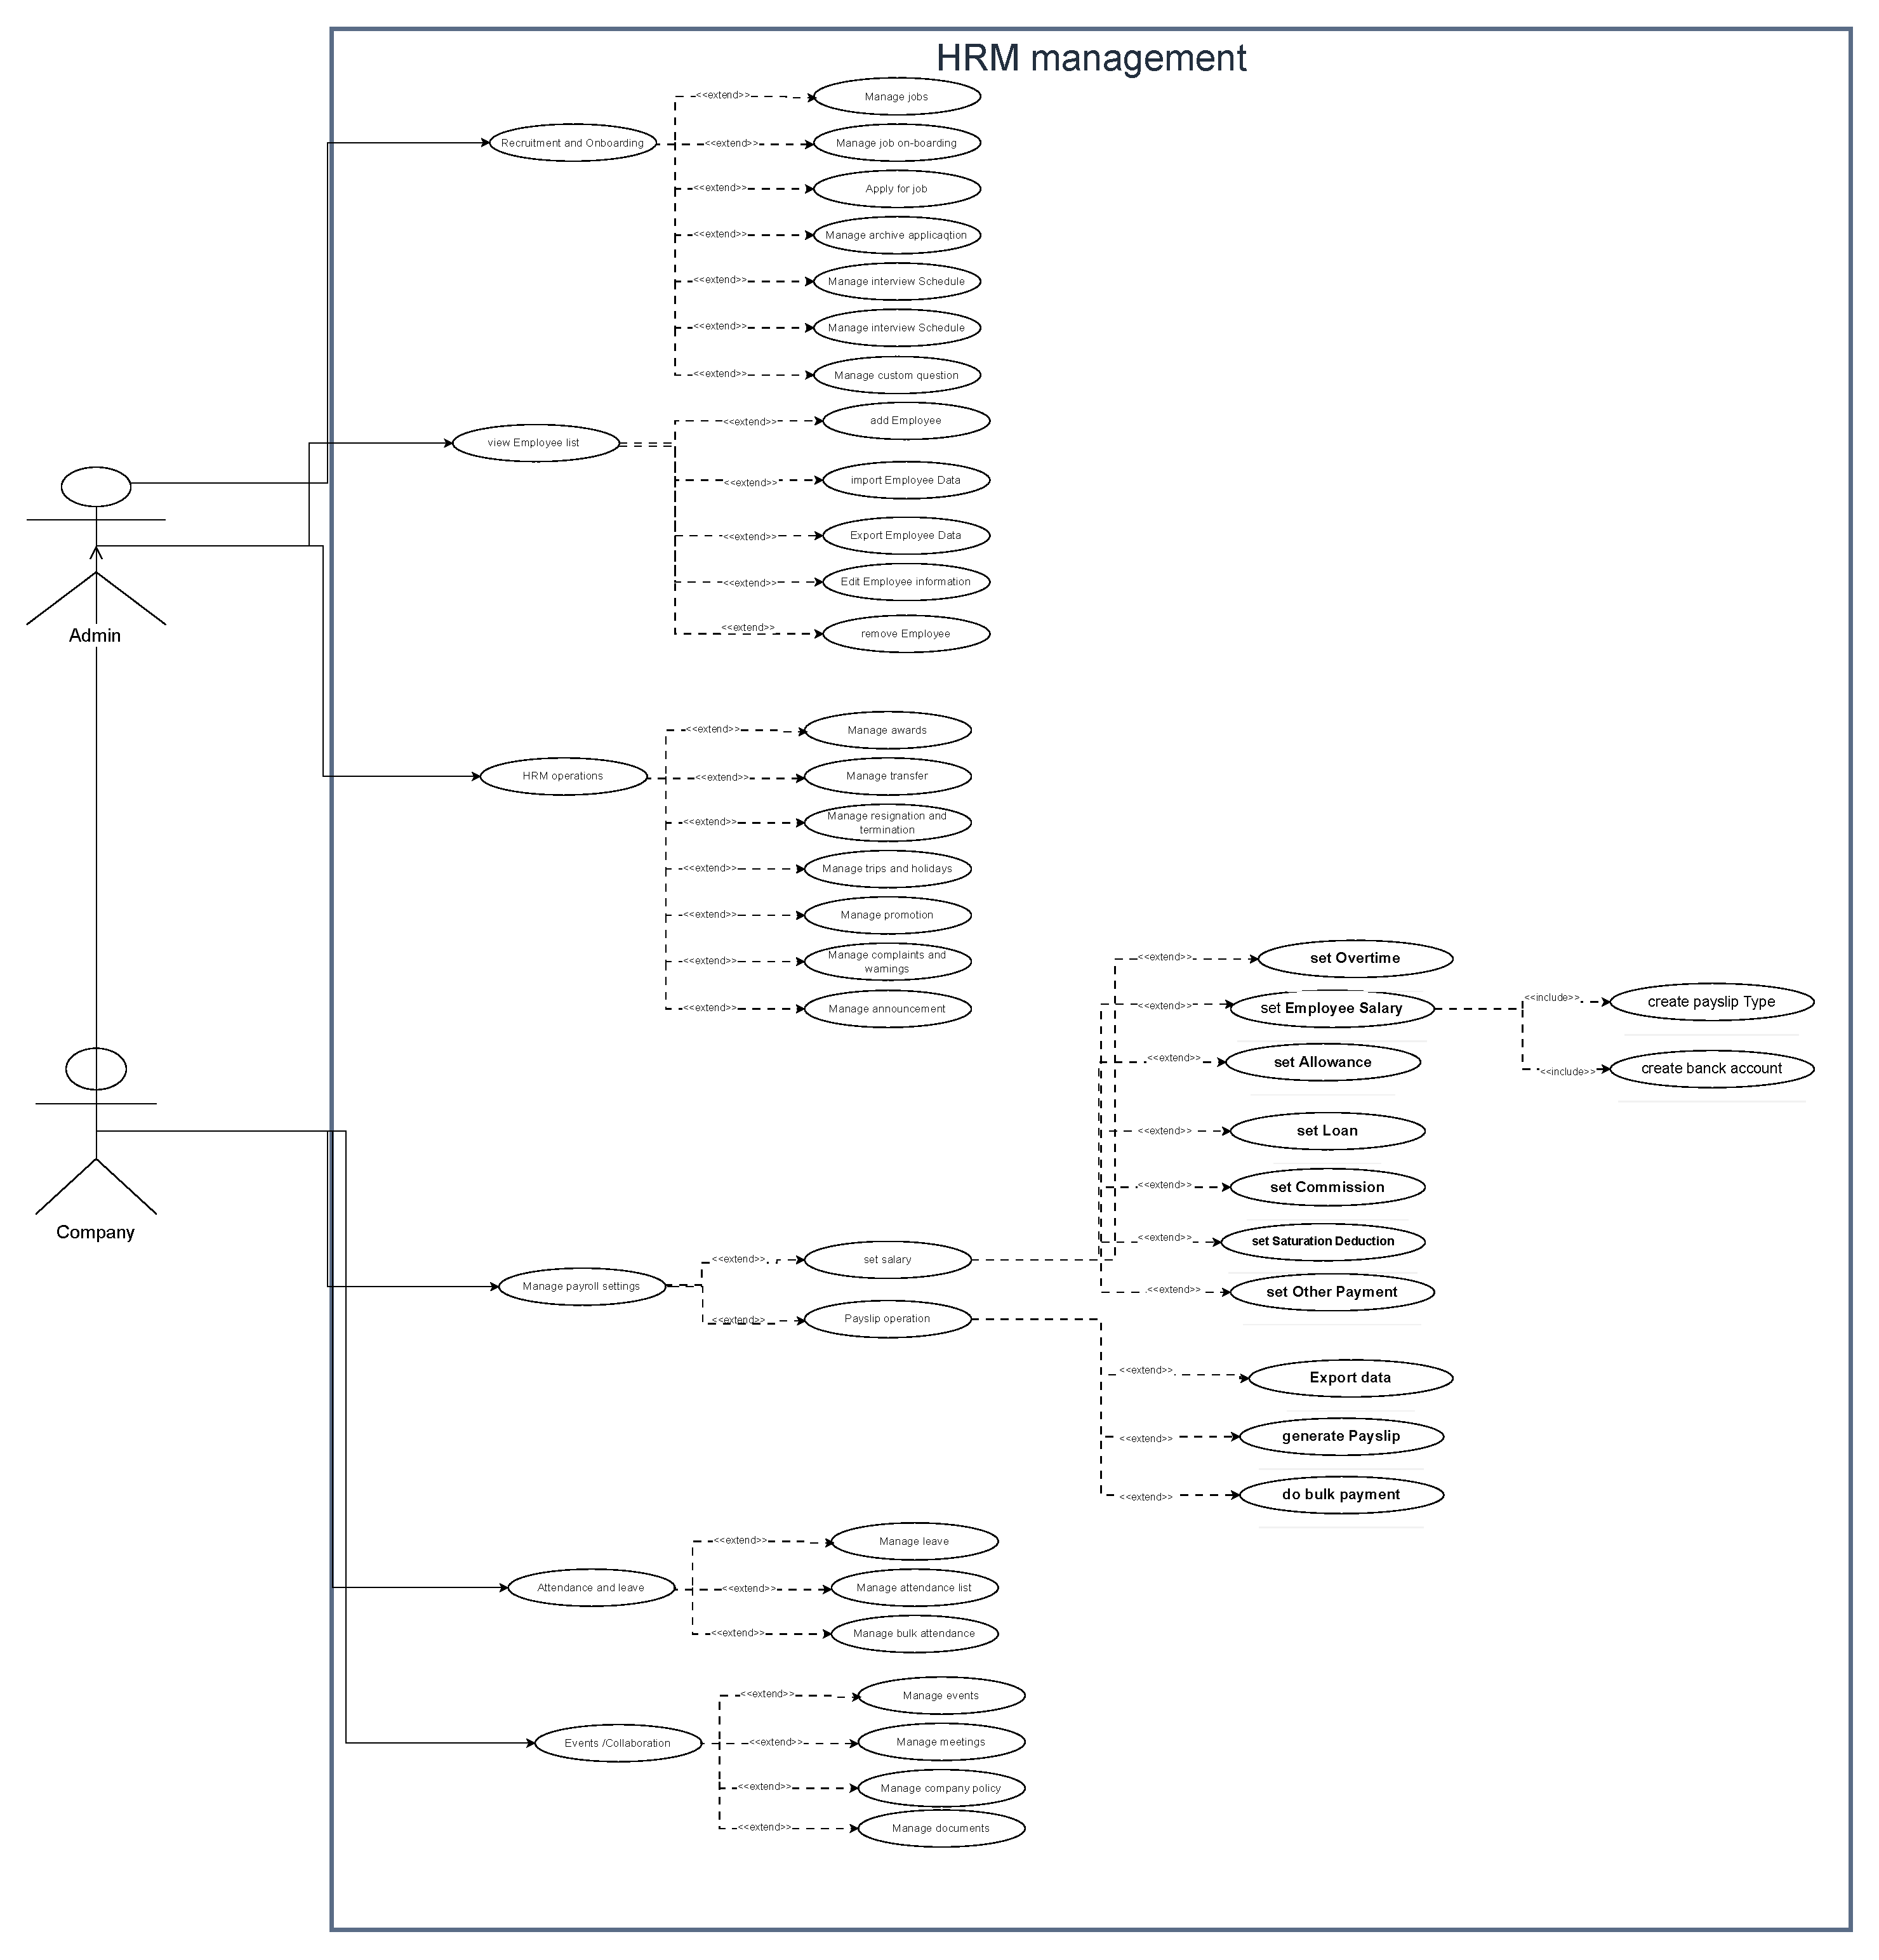
\includegraphics[width=0.9\textwidth]{chapters/chapter 3/figures/diagramGeneralUseCase (1) (1).drawio (1).pdf}
    \caption{HRM Dashboard Use Case Diagram}
    \label{fig:hrm_use_case}
\end{figure}

\subsection{Detailed Scenario: Manage Employees (HRM Dashboard)}
\begin{longtable}{|p{3cm}|p{11cm}|}
\hline
\textbf{Use Case} & Access HRM Dashboard \\
\hline
\textbf{Actor} & Admin \\
\hline
\textbf{Preconditions} &
\begin{minipage}[t]{10cm}
\begin{itemize}
    \item Admin is authenticated and has a valid JWT token.
    \item The HRM module is active.
\end{itemize}
\end{minipage} \\
\hline
\textbf{Main Flow} &
\begin{minipage}[t]{10cm}
\begin{enumerate}
    \item Admin navigates to the HRM section of the application.
    \item The system automatically sends a request: \texttt{GET /hrm-dashboard} (with JWT token in header).
    \item The system verifies the token and retrieves HRM dashboard data.
    \item The system returns a successful response containing dashboard data.
    \item The application displays the HRM dashboard to the administrator.
\end{enumerate}
\end{minipage} \\
\hline
\textbf{Alternative Flows} &
\begin{minipage}[t]{10cm}
\begin{itemize}
    \item \textbf{A1: Invalid / Missing JWT token:} System returns \texttt{401 Unauthorized}. Redirect to login.
    \item \textbf{A2: Empty Dashboard Data:} System returns \texttt{200 OK} with empty object → app displays empty dashboard.
\end{itemize}
\end{minipage} \\
\hline
\textbf{Postconditions} & 
\begin{minipage}[t]{10cm}
The HRM dashboard is successfully loaded and displayed to the authenticated Admin.
\end{minipage} \\
\hline
\caption{Use Case Scenario: Accessing the HRM Dashboard (Sprint 0)}
\label{tab:usecase_hrm_dashboard}
\end{longtable}


\subsection{Sequence Diagram: Dashboard Controller}
\begin{figure}[H]
    \centering
    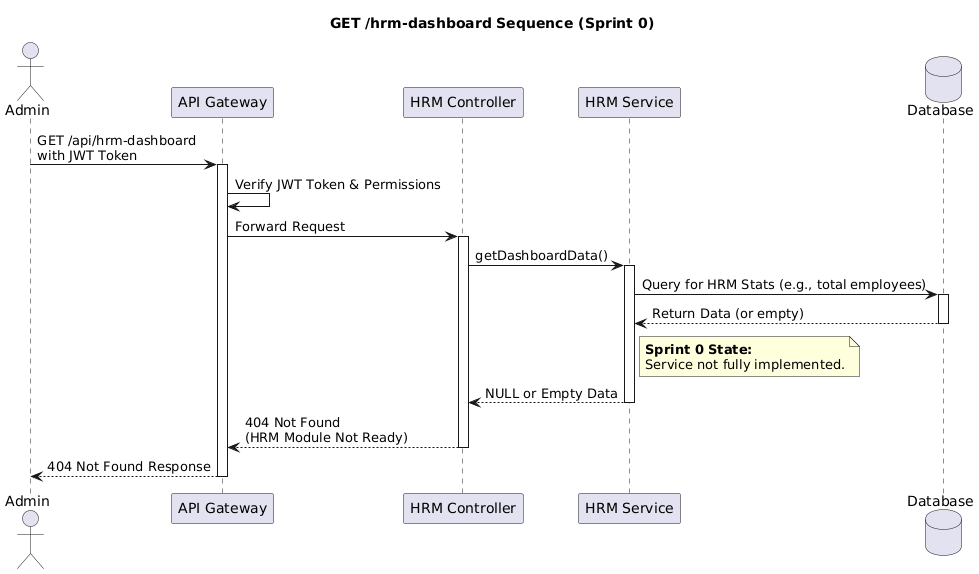
\includegraphics[width=0.9\textwidth]{chapters/chapter 3/hrmFigures/sequence_DG_hrm.png}
    \caption{Sequence Diagram for Login API}
    \label{fig:sprint0_sequence}
\end{figure}

\subsection{Class Diagram: HRM Dashboard }
\begin{figure}[H]
    \centering
    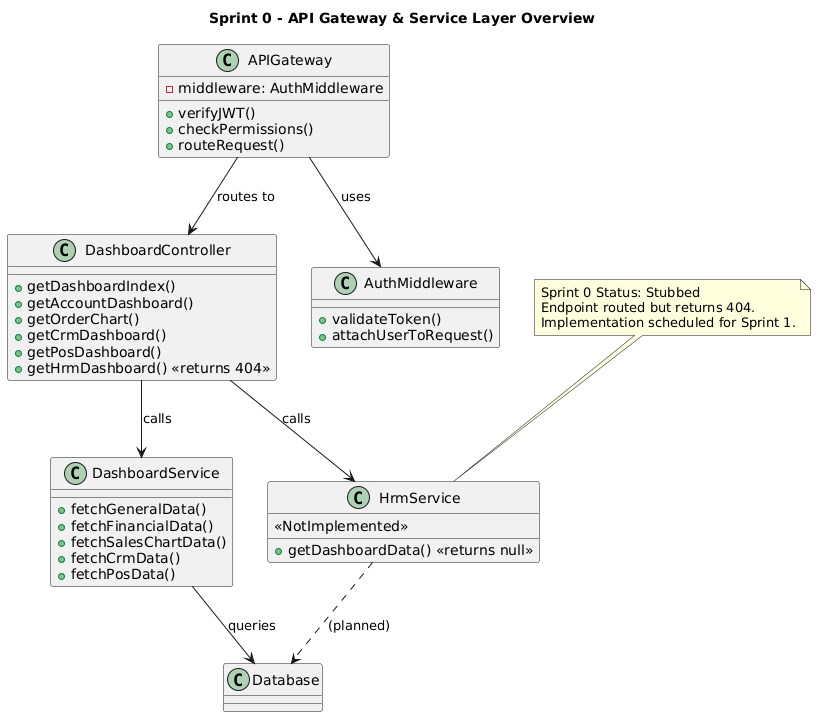
\includegraphics[width=0.85\textwidth]{chapters/chapter 3/hrmFigures/class_diagram_hrm.png}
    \caption{Class Diagram for Authentication Entities}
    \label{fig:sprint0_class}
\end{figure}

\subsection{API Testing with Postman}
To validate the core dashboard APIs implemented in Sprint 0, Postman was used for sending HTTP requests and verifying responses. The following figures illustrate the successful responses from the key endpoints, all of which require a valid JWT Bearer Token for authorization. A known issue with the HRM module is also documented.

\begin{figure}[H]
    \centering
    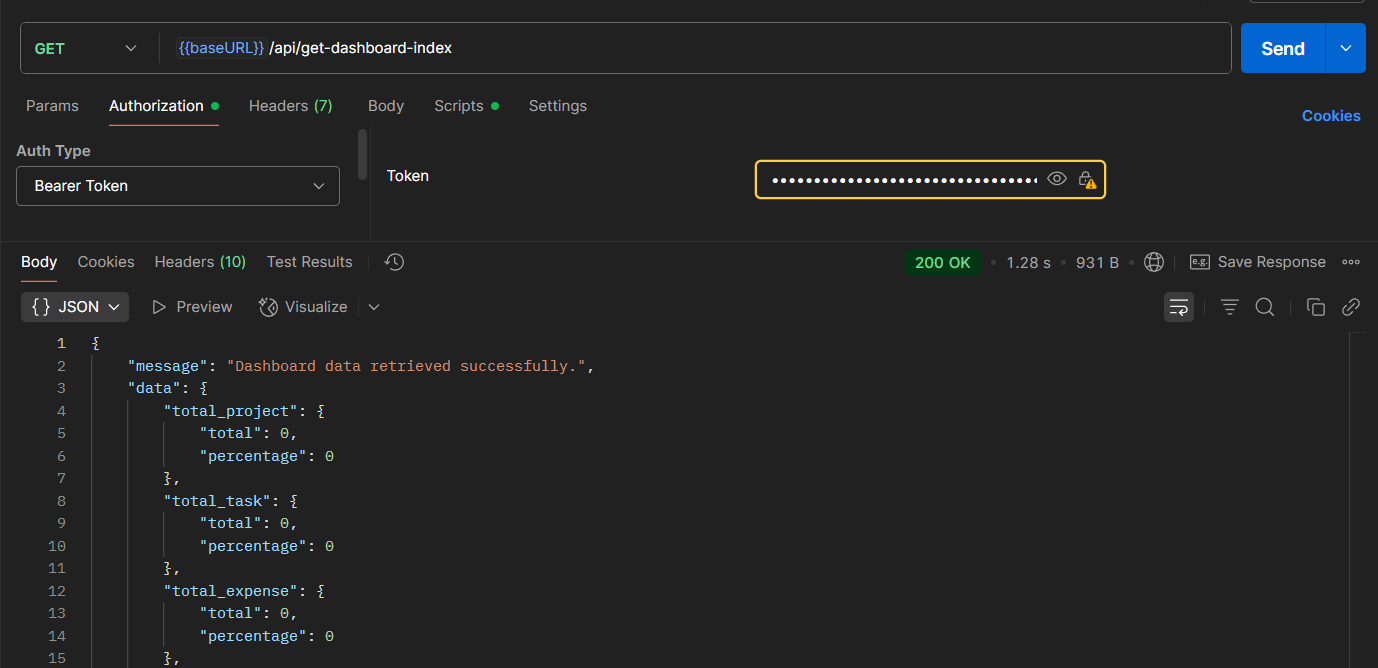
\includegraphics[width=0.8\textwidth]{chapters/chapter 3/hrmFigures/gt-dashboard-index.png}
    \caption{Postman Test -- GET /api/get-dashboard-index (Retrieving Main Dashboard Metrics)}
    \label{fig:postman_main_dashboard}
\end{figure}

\begin{figure}[H]
    \centering
    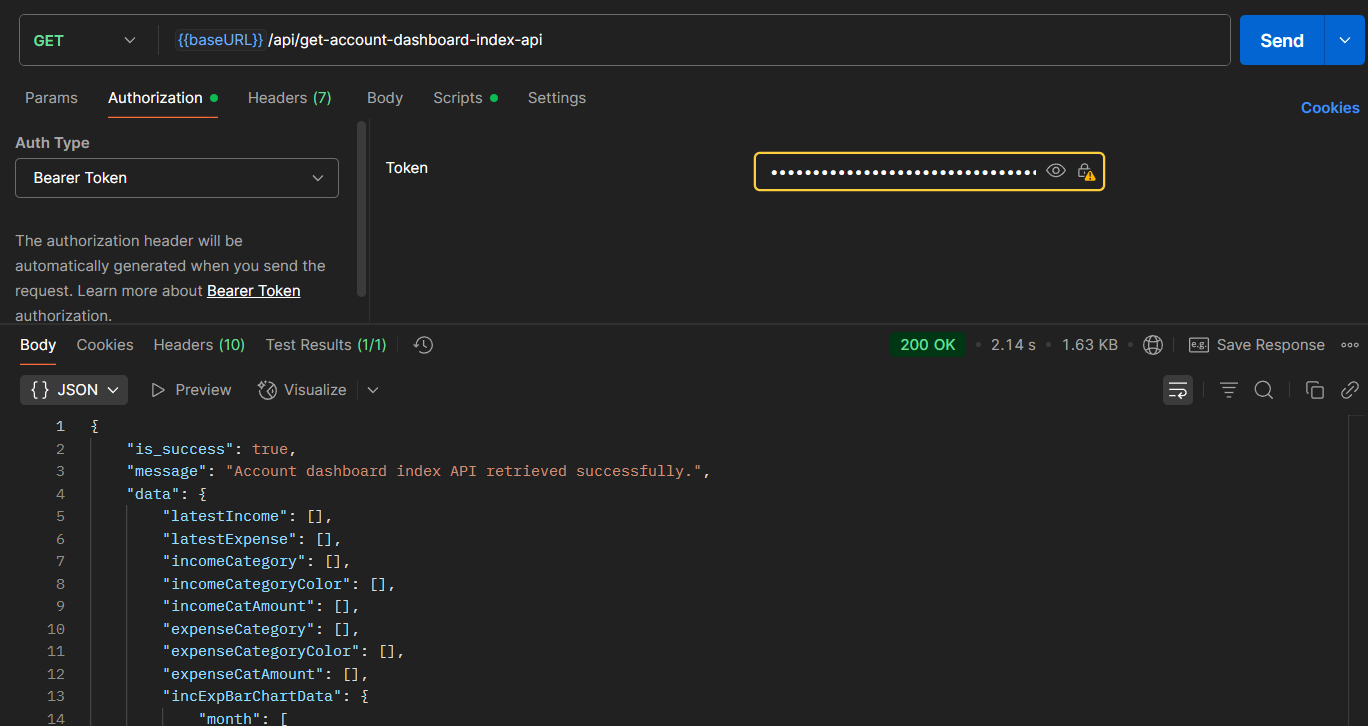
\includegraphics[width=0.8\textwidth]{chapters/chapter 3/hrmFigures/account-dashboard.png}
    \caption{Postman Test -- GET /api/get-account-dashboard-index-api (Retrieving Financial Dashboard Data)}
    \label{fig:postman_account_dashboard}
\end{figure}

\begin{figure}[H]
    \centering
    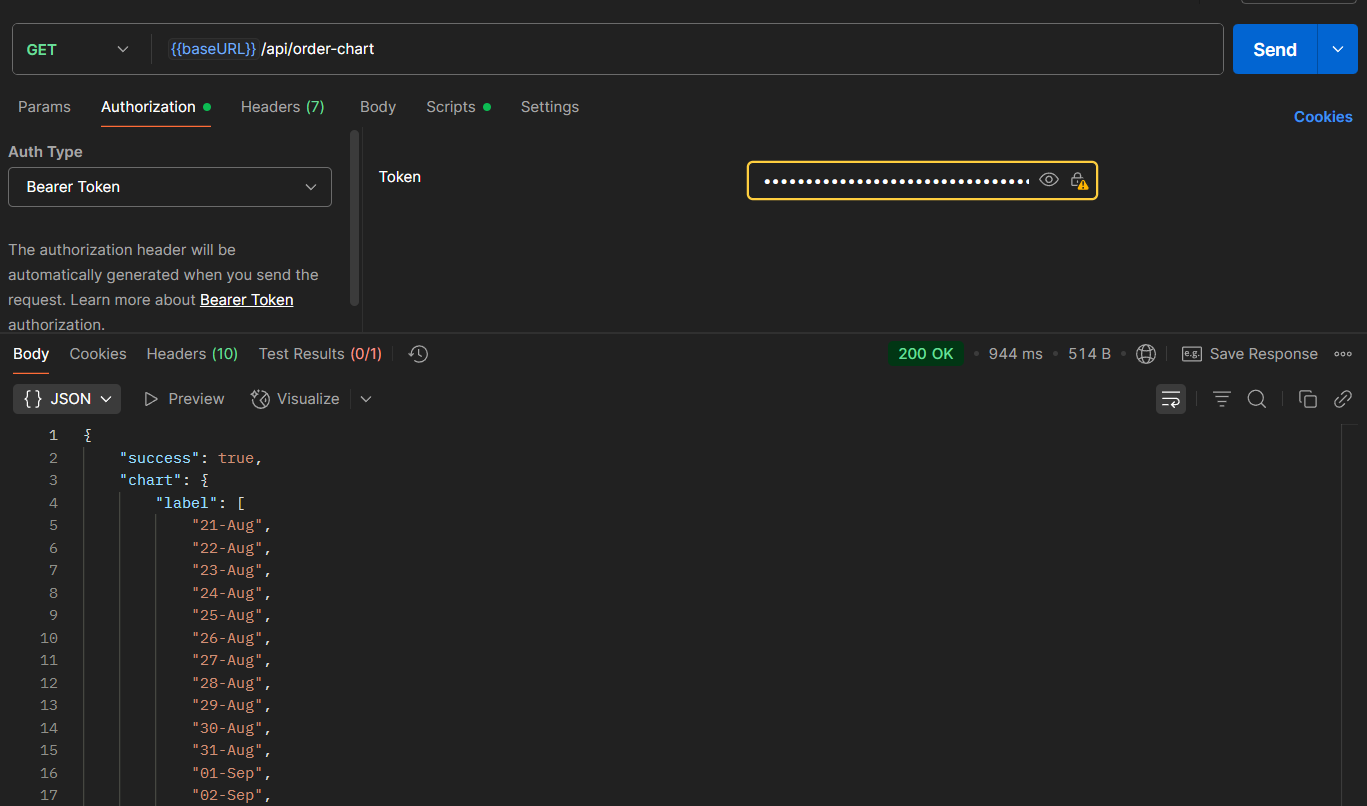
\includegraphics[width=0.8\textwidth]{chapters/chapter 3/hrmFigures/oder_chart.png}
    \caption{Postman Test -- GET /api/order-chart (Retrieving Sales Chart Data)}
    \label{fig:postman_order_chart}
\end{figure}

\begin{figure}[H]
    \centering
    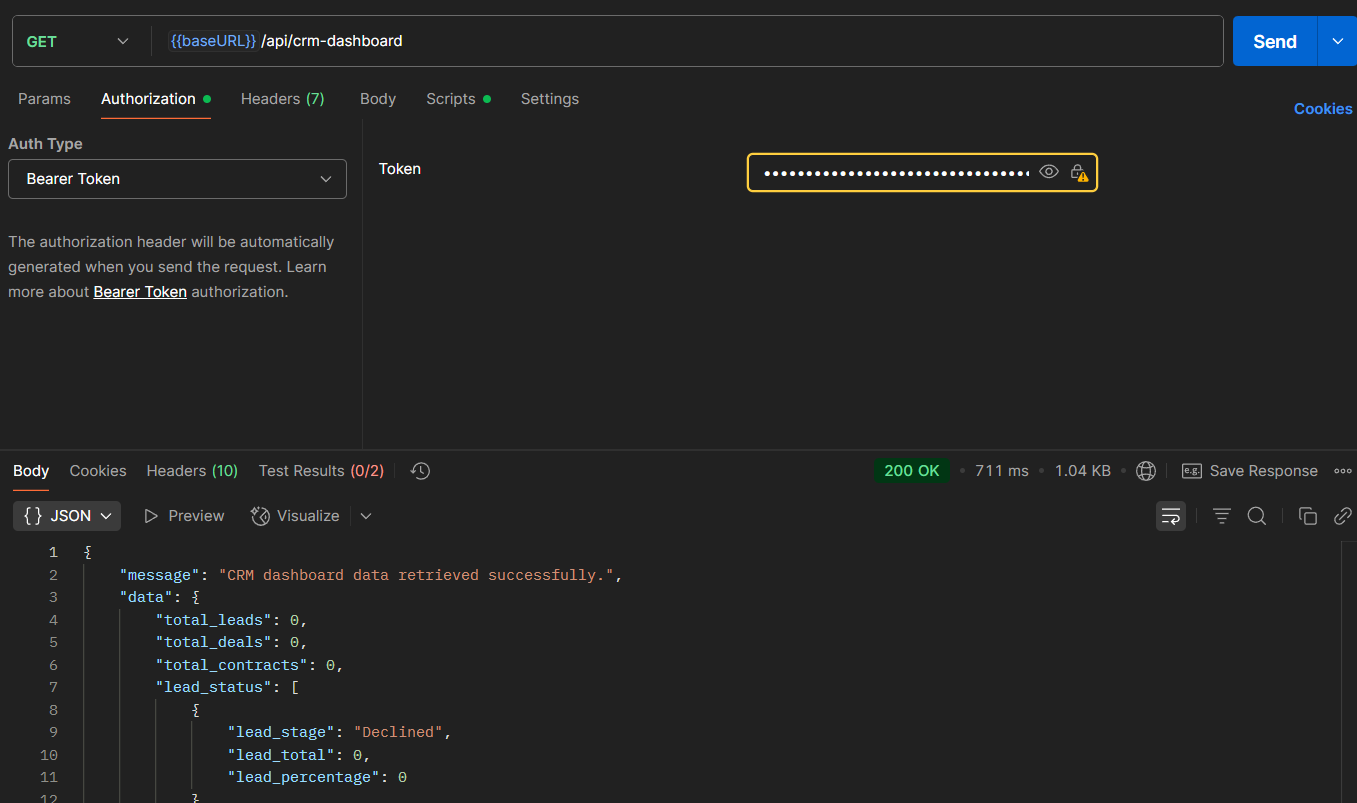
\includegraphics[width=0.8\textwidth]{chapters/chapter 3/hrmFigures/crm-dashboard.png}
    \caption{Postman Test -- GET /api/crm-dashboard (Retrieving CRM Metrics)}
    \label{fig:postman_crm_dashboard}
\end{figure}

\begin{figure}[H]
    \centering
    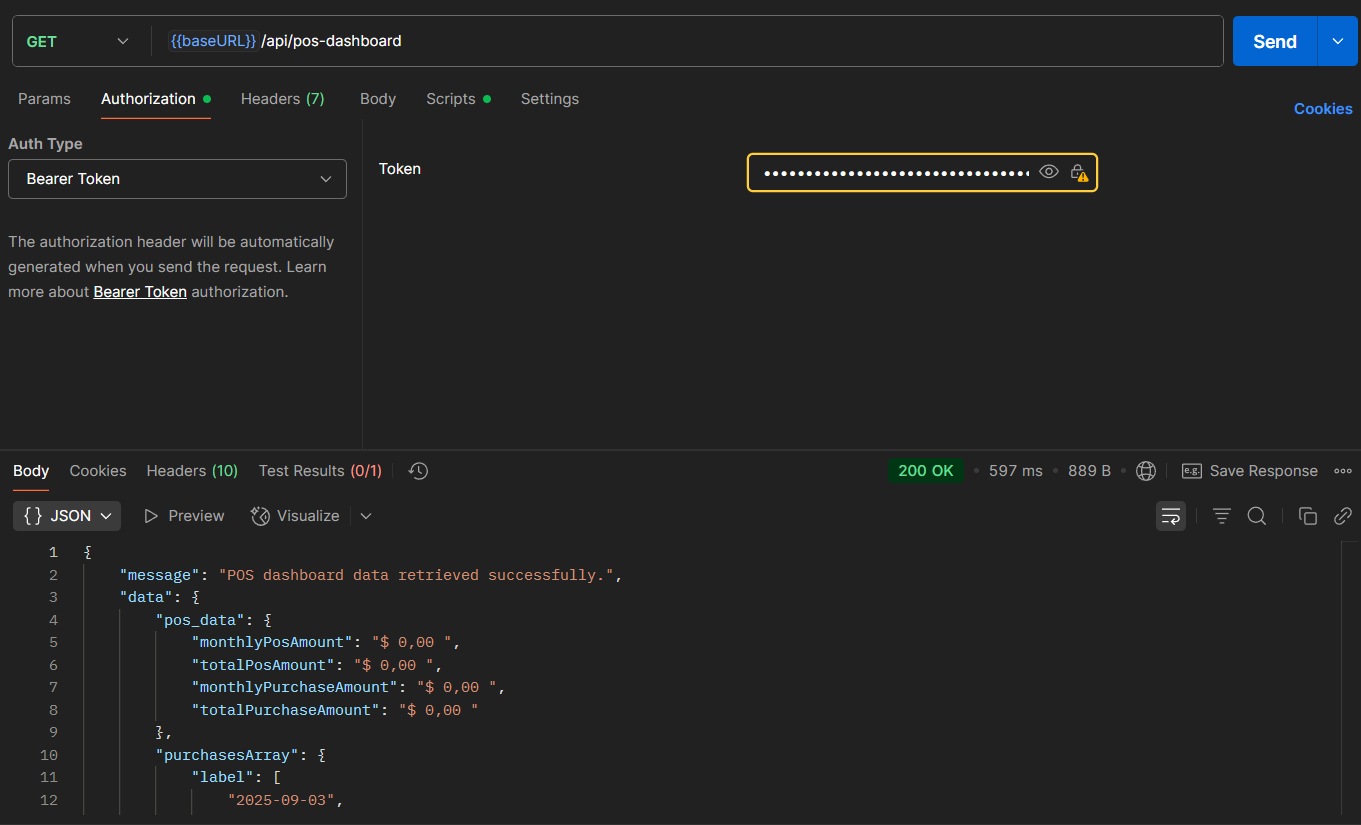
\includegraphics[width=0.8\textwidth]{chapters/chapter 3/hrmFigures/pos_dashboard.png}
    \caption{Postman Test -- GET /api/pos-dashboard (Retrieving Point-of-Sale Data)}
    \label{fig:postman_pos_dashboard}
\end{figure}

\begin{figure}[H]
    \centering
    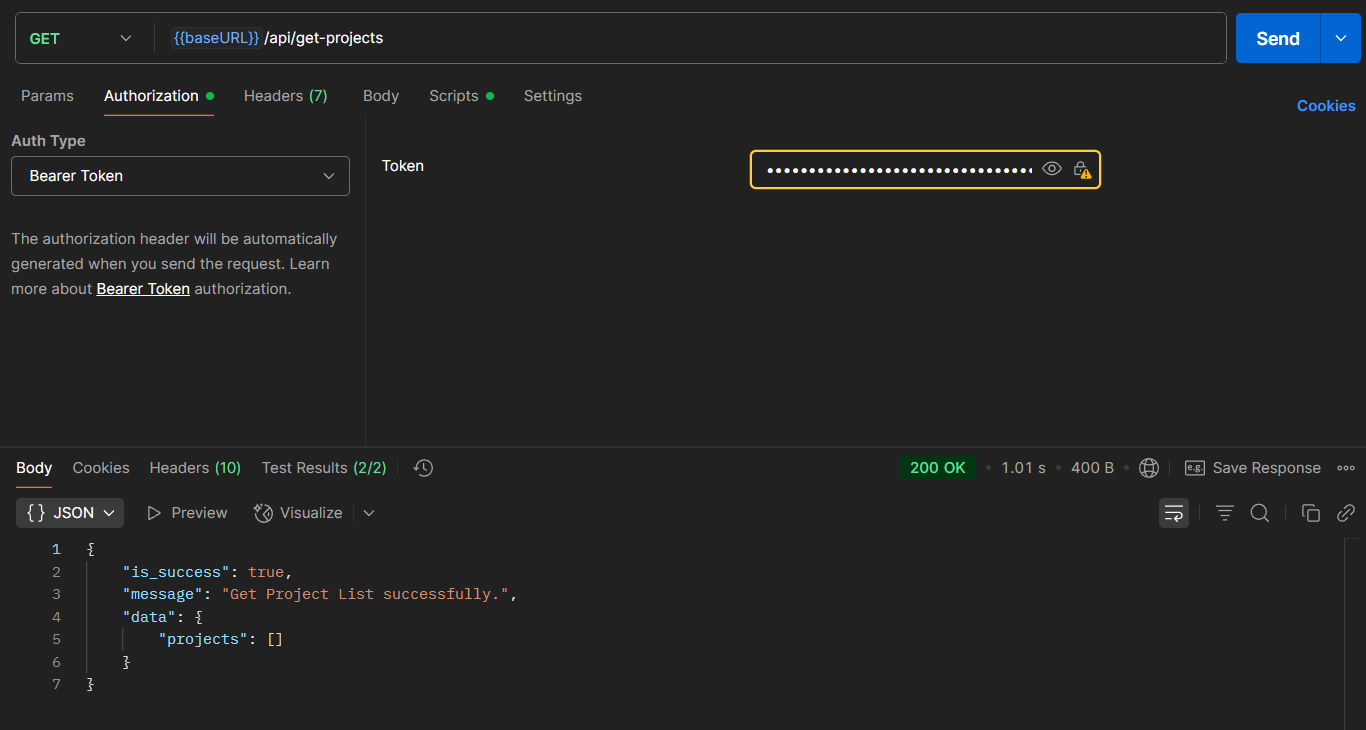
\includegraphics[width=0.8\textwidth]{chapters/chapter 3/hrmFigures/get-projects.png}
    \caption{Postman Test -- GET /api/get-projects (Retrieving Project List)}
    \label{fig:postman_get_projects}
\end{figure}

\begin{figure}[H]
    \centering
    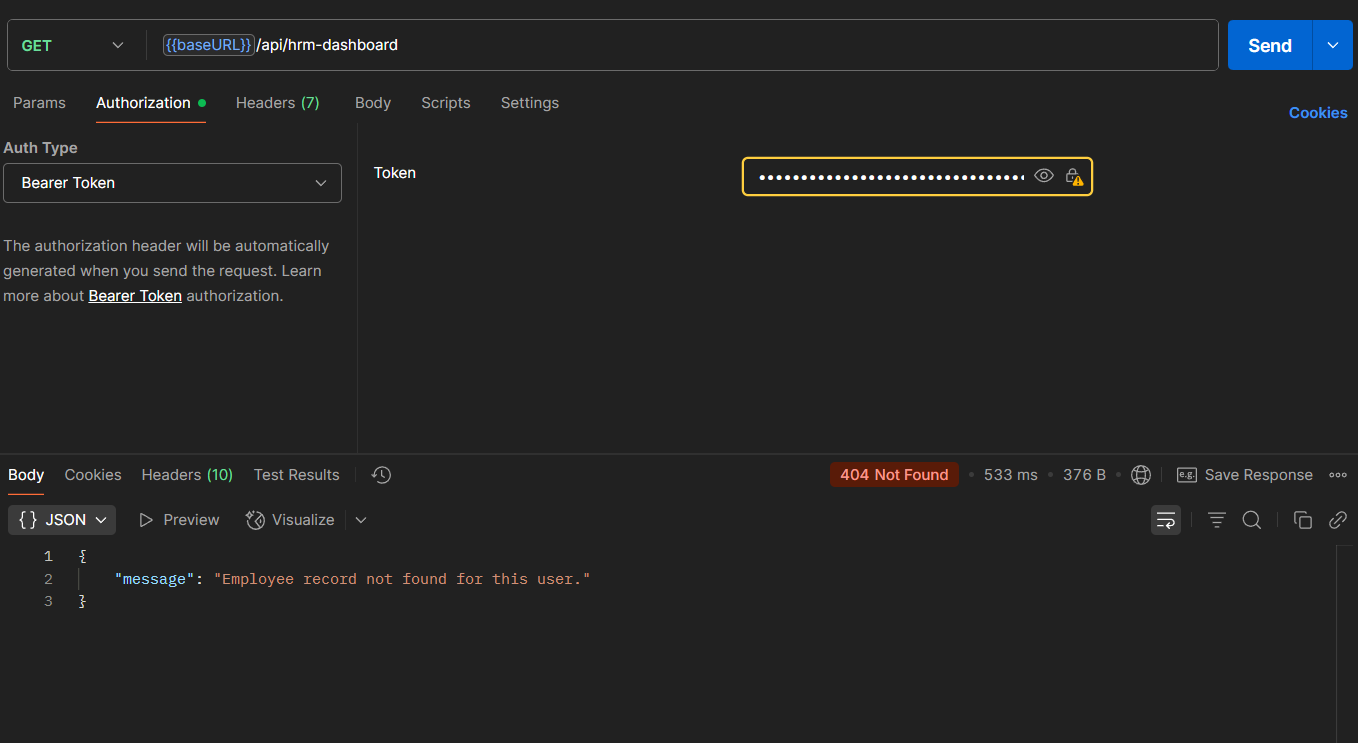
\includegraphics[width=0.8\textwidth]{chapters/chapter 3/hrmFigures/hrm_employee_not_found.png}
    \caption{Postman Test -- GET /api/hrm-dashboard (Endpoint Routed but Not Implemented - 404 Status)}
    \label{fig:postman_hrm_404}
\end{figure}

%\section{Sprint 1: Core Administrative APIs}

\subsection{Objectives}
Sprint 1 focused on building the foundational administrative APIs that define the company’s structure and workforce.  
The main goal was to implement full CRUD operations for Employees, Branches, Departments, and Designations, ensuring all entities could be created, updated, deleted, and retrieved securely.  
Bulk operations such as Import/Export for Employees were also introduced.

\subsection{Tasks Completed}
\begin{itemize}
    \item Implemented CRUD APIs for the following entities:
    \begin{itemize}
        \item Employees (with Import \& Export functionality).
        \item Branches.
        \item Departments.
        \item Designations.
    \end{itemize}
    \item Secured all endpoints with JWT authentication middleware.
    \item Documented endpoints and tested responses in Postman.
    \item Updated database schema to support relations (Employees linked to Departments, Branches, and Designations).
\end{itemize}

\subsection{Outputs}
By the end of Sprint 1, the following deliverables were achieved:
\begin{itemize}
    \item Functional APIs for organizational entities.
    \item Secure JWT-protected CRUD endpoints.
    \item Initial dataset for Employees, Branches, Departments, and Designations.
    \item Verified API responses through Postman.
\end{itemize}

% --------------------------------------------------------
% USE CASE DIAGRAM
% --------------------------------------------------------
\subsection{Administrative Use Case Diagram}
\begin{figure}[H]
    \centering
    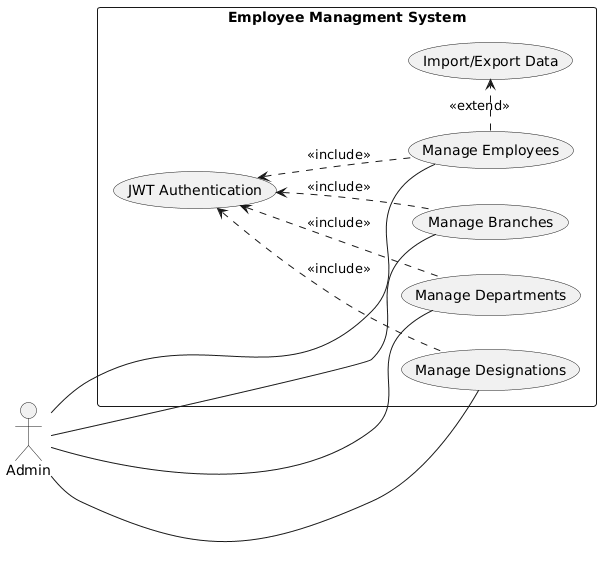
\includegraphics[width=0.85\textwidth]{chapters/chapter 3/sprint1_figures/use_case_Employee-managment.png}
    \caption{Use Case Diagram for Administrative APIs (Employees, Branches, Departments, Designations)}
    \label{fig:sprint1_usecase}
\end{figure}

% --------------------------------------------------------
% USE CASE SCENARIO TABLE
% --------------------------------------------------------
\subsection{Use Case Scenario: Create Employee}
\begin{longtable}{|p{3cm}|p{11cm}|}
\hline
\textbf{Use Case} & Create Employee Record \\
\hline
\textbf{Actor} & Admin \\
\hline
\textbf{Preconditions} & 
\begin{itemize}
    \item Admin is authenticated with a valid JWT token.
    \item The system has at least one Branch, Department, and Designation defined.
\end{itemize} \\
\hline
\textbf{Main Flow} &
\begin{enumerate}
    \item Admin selects ``Add Employee'' option in the application.
    \item System sends a \texttt{POST /employees} request with employee details (name, email, salary, branch\_id, department\_id, designation\_id).
    \item API validates request payload.
    \item API stores the new employee in the database.
    \item System returns a \texttt{201 Created} response with employee details.
\end{enumerate} \\
\hline
\textbf{Alternative Flows} &
\begin{itemize}
    \item \textbf{A1: Missing/Invalid Token:} System returns \texttt{401 Unauthorized}.
    \item \textbf{A2: Invalid Data:} System returns \texttt{422 Unprocessable Entity} with validation errors.
    \item \textbf{A3: Foreign Key Missing:} If Branch/Department/Designation ID does not exist, system returns \texttt{404 Not Found}.
\end{itemize} \\
\hline
\textbf{Postconditions} & 
\begin{itemize}
    \item A new employee record is created and stored in the database.
    \item Employee is now linked to Branch, Department, and Designation entities.
\end{itemize} \\
\hline
\caption{Use Case Scenario: Create Employee (Sprint 1)}
\label{tab:usecase_create_employee}
\end{longtable}

% --------------------------------------------------------
% SEQUENCE DIAGRAM
% --------------------------------------------------------
\subsection{Sequence Diagram: Create Employee}
\begin{figure}[H]
    \centering
    \includegraphics[width=0.9\textwidth]{}
    \caption{Sequence Diagram for Create Employee API}
    \label{fig:sprint1_sequence}
\end{figure}

% --------------------------------------------------------
% CLASS DIAGRAM
% --------------------------------------------------------
\subsection{Class Diagram: Administrative Entities}
\begin{figure}[H]
    \centering
    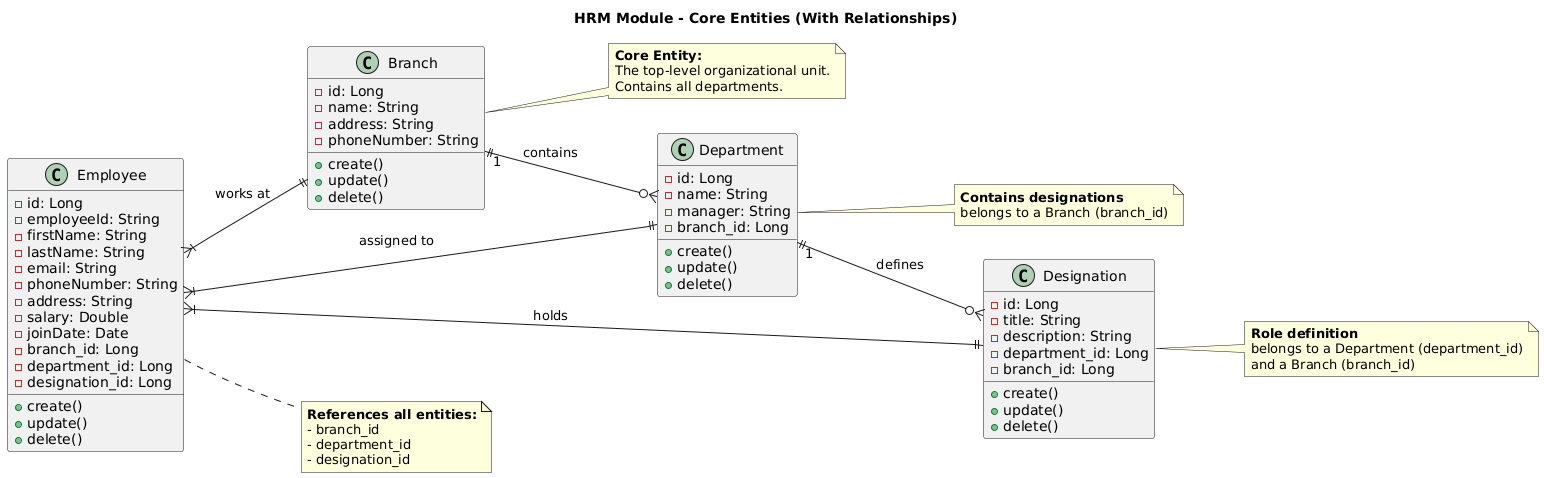
\includegraphics[width=0.85\textwidth]{chapters/chapter 3/sprint1_figures/class_diagram_s1.png}
    \caption{Class Diagram for Employees, Branches, Departments, and Designations}
    \label{fig:sprint1_class}
\end{figure}

% --------------------------------------------------------
% API TESTING WITH POSTMAN
% --------------------------------------------------------
\subsection{API Testing with Postman}
The CRUD endpoints were tested using Postman to ensure correct functionality. Below are placeholders for screenshots:

\begin{figure}[H]
    \centering
    \includegraphics[width=0.8\textwidth]{chapters/chapter 3/sprint1Figures/postman_create_employee.png}
    \caption{Postman Test -- Create Employee API}
    \label{fig:postman_create_employee}
\end{figure}

\begin{figure}[H]
    \centering
    \includegraphics[width=0.8\textwidth]{chapters/chapter 3/sprint1Figures/postman_get_employees.png}
    \caption{Postman Test -- Get All Employees API}
    \label{fig:postman_get_employees}
\end{figure}

\begin{figure}[H]
    \centering
    \includegraphics[width=0.8\textwidth]{chapters/chapter 3/sprint1Figures/postman_update_employee.png}
    \caption{Postman Test -- Update Employee API}
    \label{fig:postman_update_employee}
\end{figure}

\begin{figure}[H]
    \centering
    \includegraphics[width=0.8\textwidth]{chapters/chapter 3/sprint1Figures/postman_delete_employee.png}
    \caption{Postman Test -- Delete Employee API}
    \label{fig:postman_delete_employee}
\end{figure}

%\input{chapters/chapter3/sprint2}
%\input{chapters/chapter3/sprint3}

\section*{Conclusion}
The implementation phase transformed the specifications into a functional ERP backend system. 
Through iterative sprints, we ensured continuous progress and adaptability. 
This chapter showcased the environment setup, API development, configuration options, and reporting features, supported by UML diagrams and scenarios. 
The next chapter will evaluate the testing and validation of the developed system.

% Conclusion 
\clearpage
\chapter*{General Conclusion}
\addcontentsline{toc}{chapter}{General Conclusion}
\section*{General Conclusion}
\addcontentsline{toc}{section}{General Conclusion}

The ERP project developed for \textbf{Anter Lab} by \textit{Montassar Mejri} successfully integrates essential business processes into a unified backend system. The system offers modules for authentication, employee management, product and inventory tracking, sales (POS), and financial operations.

One of the major achievements of this project is the design and implementation of a complete \textbf{RESTful API backend} using \textbf{Laravel}, tested and documented with \textbf{Postman}, and secured with \textbf{JWT authentication}.

\textbf{Future perspectives} include:
\begin{itemize}
    \item Completing and refining the frontend layer (Next.js or mobile app).
    \item Adding advanced accounting and CRM modules.
    \item Providing detailed dashboards and business intelligence analytics.
    \item Deploying the ERP with Docker and CI/CD pipelines for scalability.
\end{itemize}

% ---------- Bibliography ----------
\clearpage
\addcontentsline{toc}{chapter}{Bibliography} % Add to TOC
\begin{thebibliography}{9}
\bibitem{laravel} Laravel Framework. \url{https://laravel.com}  
\bibitem{jwt} JWT.io — JSON Web Tokens. \url{https://jwt.io}  
\bibitem{mysql} MySQL Documentation. \url{https://dev.mysql.com}  
\bibitem{agile} Agile Methodology. \url{https://www.agilealliance.org/agile101}  
\bibitem{scrum} Scrum Framework. \url{https://www.scrum.org/resources/what-is-scrum}  
\bibitem{clickup} ClickUp — Project Management Tool. \url{https://clickup.com}  
\bibitem{uml} UML — Unified Modeling Language. \url{https://www.uml.org}  
\bibitem{php} PHP Official Documentation. \url{https://www.php.net/docs.php}  
\bibitem{laravelcrud} Laravel CRUD Tutorial. \url{https://laravel.com/docs/10.x/eloquent}  
\bibitem{restapi} REST API Principles. \url{https://restfulapi.net}  
\bibitem{postman} Postman — API Testing Tool. \url{https://www.postman.com}  
\end{thebibliography}



\end{document}